\documentclass[acmsmall]{acmart}
\usepackage{tikz}
\usepackage{amsmath}
\usepackage{filecontents}
\usepackage{algorithm}
\usepackage[noend]{algpseudocode}
\usepackage{multirow}
\usepackage{mathtools}
\usepackage{fancyvrb}
\usepackage{mdframed}
\usepackage{amsthm} 
\usepackage{microtype}
\usepackage{paralist}
\usepackage{graphicx}
\usepackage{enumitem}
\usepackage{subcaption}
\usepackage{makecell}
\usepackage{booktabs}
\usepackage{wrapfig}
\usepackage{caption}
\usepackage{subcaption}
\usepackage{listings}
% \captionsetup[figure]{belowskip=0pt}
% \captionsetup[figure]{skip=0pt}
% \captionsetup[table]{belowskip=0pt}
% \captionsetup[table]{skip=0pt}
% \setlist[enumerate]{noitemsep, topsep=0pt}
% \setlist[itemize]{noitemsep, topsep=0pt}
% \usepackage[compact]{titlesec}
% \renewcommand{\paragraph}[1]{\noindent\textbf{#1}}
% \titlespacing{\paragraph}{0pt}{*0.5}{*1}
% \setlength{\textfloatsep}{5pt plus 0pt minus 2.0pt}
% \titlespacing\section{0pt}{*1.8}{*1.1}
% \titlespacing\subsection{0pt}{*1.5}{*1.1}
% \titlespacing\subsection{0pt}{*1.3}{*0.8}
\usepackage{booktabs}
\renewcommand\footnotetextcopyrightpermission[1]{} % 
\renewcommand\footnotetextcopyrightpermission[1]{} 
\setcopyright{none}
\settopmatter{printacmref=false, printccs=false, printfolios=true}
\acmDOI{}
\acmISBN{}
\acmConference[Submitted for review to SIGCOMM]{}
\acmYear{2025}
\acmPrice{}

\begin{document}
	%-------------------------------------------------------------------------------


	\title[CAP]{CAP: Detecting Network Device Misconfigurations with Context-Aware Prompting of LLMs}
		\author{Paper \#1257, \pageref{endOfBody} pages body, 19 pages total}
        %!TEX root = main.tex
%!TEX spellcheck = en_US

\begin{abstract}

Verifying network configurations is critical for ensuring operational stability, but traditional tools force a trade-off between the high manual effort of model checkers and the semantic shallowness of consistency checkers. While Large Language Models (LLMs) are a promising alternative, naive approaches like full-file, partition-based, or chain-of-thought prompting fail to handle the large, interconnected nature of configuration files, leading to context overload or fragmentation.
We introduce the Context-Aware Prompting (\sysname{}) framework, which enables an LLM to reason about network configurations like a human expert. \sysname{} first performs comprehensive context mining, identifying all potentially relevant neighboring, similar, and referenced (both intra- and cross-device) configurations. It then engages the LLM in a structured, interactive dialogue, where the model first requests the specific context it needs before performing its final, focused analysis. This on-demand approach provides the necessary context for deep reasoning while avoiding overload.
Our evaluation on production network configurations demonstrates that \sysname{} achieves near-perfect accuracy on known misconfigurations and uncovers over 20 previously undetected, real-world errors. We show that \sysname{} significantly outperforms existing tools and that the choice of LLM backend reveals a crucial precision-recall trade-off. Ultimately, \sysname{} provides a more effective and scalable paradigm for LLM-based network verification.

\end{abstract}

		\newcommand{\chase}[1]{\textcolor{blue}{[#1]}}
		\newcommand{\eg}{{\it e.g.}}
		\newcommand{\ie}{{\it i.e.}}
		\newcommand{\aaron}[1]{{\color{teal}{(Aaron: #1)}}}
		\newcommand{\mypara}[1]{\vspace{0.05cm}\noindent{\bf {#1}}}
		\newcommand{\mysubpara}[1]{\vspace{0.05cm}\noindent{\textit{#1}}}
		\newcommand{\etal}{{\it et al.}}
		\newcommand{\sysname}{{CAP}}
		\newlength{\oldintextsep}
		\setlength{\oldintextsep}{\intextsep}
		\setlength\intextsep{0pt}

        		\maketitle

%!TEX root = main.tex
%!TEX spellcheck = en_US

\section{Introduction}
\label{sec:intro}

Ensuring the stability, security, and performance of network infrastructures
requires carefully configuring routers, switches, firewalls, etc. A misconfiguration on even a single network device can lead to black holes, unintended network access, inefficient routes, and a range of other issues~\cite{gill2011understanding, turner2010california}.

Although some configuration tasks are automated---especially in large networks~\cite{tian2019jinjing, ramanathan2023aura, mahimkar2022aurora, rasche2023esnet, gember-jacobson2015mpa}---many (changes to) configurations are manually written by human experts~\cite{abhashkumar2020aed}. Network engineers rely on extensive knowledge gained from years of experience with an organization's network(s), vast vendor documentation~\cite{ciscosupport, junosdocumentation}, industry best practices~\cite{manrs}, etc. To avoid problems, engineers must consider the interplay between (a change to) a configuration and related aspects of devices' configurations. This is challenging for humans, because even a single device's configuration is often hundreds or thousands of lines long with many dependencies between segments~\cite{benson2009complexitymetrics}.


Researchers and practitioners have developed numerous network configuration verifiers to address this challenge.
{\em Model checkers}~\cite{fogel2015general, beckett2017general, abhashkumar2020tiramisu, prabhu2020plankton, zhang2022sre, steffen2020netdice, ye2020hoyan, ritchey2000using,al2011configchecker, jeffrey2009model, batfish} analyze network-wide forwarding behaviors under various scenarios (\eg, link failures) to detect violations of network objectives (\eg, reachability). These tools rely on
%Tool developers must implement 
algorithms or formalisms that codify protocol- and vendor-specific configuration semantics as well as network-specific forwarding policies. These require significant manual effort to define---only some algorithms and policies can be automatically inferred~\cite{birkner2020config2spec, kheradmand2020anime, sharma2023prosper}---and are difficult to define correctly and completely~\cite{ye2020hoyan, birkner2021metha}; hence, model checkers have a high overhead to adoption.
{\em Consistency checkers}~\cite{kakarla2024diffy,kakarla2020finding, le2006minerals, feamster2005detecting, tang2021campion, le2008detecting, le2006characterization, batfish}, on the other hand, compare configurations across devices or against best-practices and flag deviations as potential issues.
% While this statistics-driven approach requires minimal manual effort, it lacks semantic depth.
While these statistics- or rule-driven approaches require minimal manual effort, they lack semantic depth and the ability to reason about intentional deviations.
For example, a consistency checker might flag a rarely used packet filter, even though the filter is required in some contexts to satisfy security objectives.


Large language models (LLMs)~\cite{deepseekai2024deepseekv3technicalreport, achiam2023gpt} offer a promising avenue to avoid the classic trade-off between semantic depth and ease-of-use in network verification. Pretrained on a vast, public corpus of data that includes protocol specifications and vendor documentation, LLMs develop a deep understanding of general network configuration principles. When presented with a specific, previously unseen device configuration at inference time, the LLM applies this broad knowledge to effectively translate the configuration into a reasoned judgment. This process hinges on the model's self-attention mechanism, which mathematically weighs the importance of every token in the configuration relative to every other token. By using attention, the model builds a rich, contextual map, understanding, for instance, that a specific access control list on line 50 directly impacts an interface definition on line 450. After creating this complex, attention-weighted internal representation, the model’s final layers distill it into a simple, probabilistic choice over a small set of output tokens, such as 'true' or 'false'. This ability to use attention to interpret complex dependencies and then collapse that understanding into a discrete assessment makes LLMs analogous to human experts applying broad domain knowledge to diagnose a specific problem.

However, recent efforts to leverage LLMs for configuration analysis~\cite{bogdanov2024leveraging,wang2024identifying,liu2024large, wang2024netconfeval, lian2023configuration} have missed an important insight:
human engineers do not examine entire configurations in a rigid, linear fashion; instead, engineers identify relevant configuration lines and dynamically ``jump'' to related parts of the configuration. Similarly, LLMs are more effective when provided with {\em concise, relevant context} that mirrors this human approach. Feeding an LLM the entire configuration at once risks exceeding token limits, and splitting configurations into arbitrary partitions~\cite{lian2023configuration} can obscure dependencies between different parts. Furthermore, overloading the model with irrelevant or excessive information can dilute its reasoning capabilities~\cite{lican,li2024long,qian2024long}, much like a human struggling to recall long-past details. We discuss these issues in more depth in Section~\ref{sec:background:context}.

The central challenge, therefore, is to bridge the gap between the reasoning capabilities of LLMs and the complex, interdependent nature of network configurations. An effective framework must enable an LLM to analyze configurations in a way that is both semantically deep and scalable, mirroring a human expert's ability to dynamically seek out relevant context without being overwhelmed by the sheer volume of a full configuration file.
In this paper, we propose the Context-Aware Prompting (\sysname{}) framework, a holistic solution that addresses this challenge through two integrated components:

\mypara{1. Automatic and Accurate Context Mining:}
To ground the LLM's reasoning, \sysname{} first performs automated context extraction. We model the configuration's nested structure as a hierarchical tree, where configuration stanzas and parameters (\eg, interface GE1/1/1) are intermediate nodes and terminal commands (\eg, mtu 9000) are leaf nodes. This structure enables the systematic identification of key context categories—neighboring, similar, and referenced configuration lines—ensuring a concise yet sufficient corpus is available for analysis. Furthermore, we distinguish pre-defined from user-defined values using an initial LLM query to classify the terminal value in a given line.

\mypara{2. Guided Interactive Prompting for Context Management:}
To prevent context overload and focus the model's attention, \sysname{} introduces an guided, interactive dialogue. While modern LLMs have large context windows, providing excessive or unfocused information is known to degrade reasoning quality, an issue distinct from hard token limits. Our framework mitigates this by having the LLM first explicitly request only the specific context it needs from the categories mined in the first component. This allows the model to incrementally build its understanding and enables more precise detection.


We evaluate \sysname{} on configurations from three diverse networks (Internet2 and two university campuses), structuring our analysis around four key questions. Our evaluation demonstrates that (1) \sysname{} achieves 100\% accuracy in detecting a wide range of known synthetic and real-world misconfigurations; (2) it can uncover novel, previously unknown issues in production networks, while also highlighting the challenge of false positives with some LLM backends; (3) the choice of LLM significantly impacts reasoning strategies and outcomes; and (4) \sysname{} substantially outperforms existing model checkers and consistency-based tools on a controlled set of complex errors.
\section{Motivation}
\label{sec_motivation}
\label{sec:motivation}

\begin{wrapfigure}{r}{0.45\columnwidth}
\footnotesize
\begin{lstlisting}[basicstyle=\tiny, numbers=left, lineskip=0pt, frame=single, xleftmargin=2em, framexleftmargin=1.5em, numbersep=0.5em, basewidth=0.52em]
interfaces {
    ge-0/0/1 {
        mtu 1500;
        unit 0 {
            family inet {
                address 10.0.1.1/24;
                filter { input EXAMPLE-FILTER; }
...
    ge-0/0/2 {
        mtu 9000;
        unit 0 {
            family inet {
                address 10.0.2.1/24;
                filter { input EXAMPLE-FILTER; }
...
protocols {
    bgp {
        group EBGP-PEER {
            type external;
            peer-as 65002;
            neighbor 10.0.2.2;
...
firewall {
    family inet {
        filter EXAMPLE-FILTER {
            term ALLOW-INTERNAL {
                from { source-address 10.0.0.0/16; }
                then { accept; }
            }
...
\end{lstlisting}
\caption{Example device configuration in Junos OS}
\label{fig:example_config}
\end{wrapfigure}

Ensuring network configurations are correct is a critical but notoriously difficult task. 
Configurations possess a formal, nested structure---as shown in Figure~\ref{fig:example_config}---where settings are logically nested within specific blocks---\eg, an MTU is specified (line 3) within an interface stanza (lines 2-7). However, configurations are also woven together by a web of critical, non-hierarchical relationships where part of a device's configuration refers to another part of the configuration---\eg, an interface block references a packet filter (line 7) defined in a separate block (lines 25-29)---or another device's configuration---\eg, a BGP neighbor statement (line 21) references the address configured in another device's interface (not shown)~\cite{benson2009complexitymetrics, maltz2004routing}.
%For example, Figure~\ref{fig:example_config} shows an example of a portion of a single device's configuration in Junos OS format.
Furthermore, configurations are often immense---typically hundreds to thousands of lines per device~\cite{benson2011evolution, feamster2005detecting}---and differ syntactically and semantically between vendors~\cite{benson2009complexitymetrics, tang2021campion, ye2020hoyan}.
% An effective verifier must therefore be able to understand not just the explicit, nested structure, but also these implicit, reference-based dependencies. \aaron{The preceding requirements for an effective verifiers emphasize configuration {\em structure}, but a proponent of model checkers would likely argue that {\em semantics} are important. One way to distinguish model checkers and consistency checkers is that the former focuses primarily on configuration semantics while the later focuses primarily on configuration structure. LLMs seem to strike a middle ground, considering both semantics and structure---although LLMs are really just learning patterns, which is a matter of structure and not semantics.} This complexity has led to various verification paradigms, each with distinct trade-offs.
An effective verifier must therefore be able to reason about both the configuration's structure (its syntax and patterns) and its semantics (the resulting network behavior). This dual requirement has led to different verification paradigms, each with distinct trade-offs.

Researchers and practitioners have developed two primary types of network configuration verifiers. {\em Model checkers}~\cite{fogel2015general, batfish} focus on semantics: they analyze logical models of network-wide forwarding behavior to detect violations of high-level objectives (\eg, reachability), but this requires significant manual effort to define and maintain the necessary formal policies~\cite{ye2020hoyan}. In contrast, {\em consistency checkers}~\cite{kakarla2024diffy, le2006minerals} focus on structure: they compare configurations against pre-defined or inferred patterns to flag deviations, but their lack of semantic understanding often leads them to flag valid, intentional customizations as errors.

Large Language Models (LLMs) offer a promising way to bridge this gap. An LLM appears to handle both structure and semantics; however, its understanding of semantics is an emergent property learned from modeling the statistical patterns (\eg, the structure) of vast amounts of text. This unique position is why LLMs are a powerful new tool for this domain.


\subsection{Why LLMs?}
\label{sec:motivation:llms}

Recent work has shown Large Language Models (LLMs) are a promising avenue for generating network configurations~\cite{wang2024netconfeval, bogdanov2024leveraging, mondal2023what, wang2023making, li2024preconfig} and analyzing system configurations~\cite{lian2023configuration, wang2024identifying}. LLMs' suitability for these tasks stems from: (1) LLMs' broad ``understanding'' of network configuration developed through extensive pretraining on vast datasets,
%that include protocol specifications, vendor documentation, Q\&A forums, etc.; 
and (2) LLMs' context-aware reasoning that combines user prompts (e.g., configuration snippets and questions) with pretrained knowledge to generate responses (e.g., assessments of configuration correctness).

    
\mypara{Broad knowledge of network configuration developed through pretraining:} 
Transformer-based generative LLMs~\cite{vaswani2017attention,hill2024transformers,lin2022survey} 
 develop a deep, contextual understanding of configurations during pretraining by processing extensive datasets that include protocol specifications, vendor documentation, Q\&A forum posts, etc.
%documentation, specifications, and configurations from a variety of sources (e.g., vendors, standards bodies, Q\&A forums)
\cite{qiu2020pre,achiam2023gpt,touvron2023llama,brown2020language}. 
Structural hierarchies, semantic relationships, and statistical patterns in configurations are embedded within the model’s parameters using positional encodings---which characterize sequences of tokens (e.g., parts of configuration commands)---and multi-head self-attention mechanisms---which dynamically prioritize critical tokens (\eg, subnet addresses, permit/deny actions). For example, the model's parameters encode routing policy formats, relationships between routing policies and routing protocols, and routing policy best practices. In other words, the model is a probabilistic repository of knowledge akin to a human engineer's conceptual model of configurations.


\mypara{Integrating prompts and pretrained knowledge for context-aware reasoning:}
When a user provides configuration snippets and instructions in a prompt (\eg, ``evaluate this ACL for conflicts''), an LLM combines its pre-trained knowledge with the contextual information in the prompt. The self-attention mechanism enables the model to cross-reference tokens in the prompt with its stored knowledge, such as identifying a conflict between a firewall rule and routing policy based on probabilistic relationships learned during training. By estimating the likelihood of each token or sequence (\(p(\text{token}_i \mid \text{token}_1, \ldots, \text{token}_{i-1})\)), the model highlights deviations from high-probability patterns, flagging potential misconfigurations such as overlapping address ranges or misplaced \texttt{deny} directives. This integration mirrors how a human engineer draws on their knowledge and experience to evaluate configurations and apply abstract principles to specific cases.

\mypara{Core LLM Capabilities for Structured Languages:}
The suitability of LLMs for configuration tasks is analogous to their well-established success in code analysis and generation. Network configurations, much like programming code, are formal languages that possess three key properties LLMs are adept at learning: (1) a rigid syntax and grammatical structure; (2) a hierarchical organization of nested blocks and stanzas; and (3) critical long-range dependencies, where a definition in one area impacts behavior many lines away. The Transformer architecture is the primary reason for this effectiveness, as its core mechanisms are designed to model exactly these properties. Specifically, positional encodings allow the model to learn the strict sequential order and hierarchical structure inherent in the syntax, while the self-attention mechanism enables every token to directly attend to every other token, regardless of their distance. This allows the model to effectively capture the long-range dependencies common in both code and configurations, such as linking a policy's application to its distant definition.

\mypara{Advantages over non-LLM-based network verifiers:} %LLMs' extensive pretraining and context-aware reasoning 
The aforementioned features make LLMs easier to use and more widely applicable than network verifiers based on model checking or consistency checking. 

Model checkers~\cite{fogel2015general, beckett2017general, abhashkumar2020tiramisu, prabhu2020plankton, zhang2022sre, steffen2020netdice, ye2020hoyan, ritchey2000using,al2011configchecker, jeffrey2009model, batfish}---which create and analyze logical models of network behavior to verify compliance with network requirements---heavily rely on the manual specification of algorithms and policies. These are hard to define correctly and completely~\cite{ye2020hoyan, birkner2021metha}, even with the assistance of other tools~\cite{birkner2020config2spec, kheradmand2020anime, sharma2023prosper}. 
% In contrast, LLMs are fully automated, requiring no human-defined rules and dynamically adapting to new contexts. \aaron{Is it well known that LLMs can ``dynamically adapt to new contexts''? Do we need some citations to backup this claim?} 
In contrast, LLMs require no human-defined rules for specific tasks, leveraging their ability for in-context learning~\cite{brown2020language} to adapt to the provided configuration. 
This makes LLMs better suited for analyzing configurations involving vendor-specific nuances  or un(der)specified network requirements. 
For example, an LLM trained on public documentation may correctly interpret a Juniper-specific `apply-groups' directive—a non-standard inheritance mechanism—that a generic, protocol-based model checker would miss, especially when the framework provides it with the concise, relevant context of the group being applied.
One caveat is that LLMs' reliance on probabilistic reasoning prevents them from computing precise forwarding behaviors in some scenarios, so networks with well-specified or stringent requirements may choose to use model checkers in tandem with LLMs.





Consistency checkers~\cite{kakarla2024diffy,kakarla2020finding, le2006minerals, feamster2005detecting, tang2021campion, le2008detecting, le2006characterization, batfish}---which analyze patterns in the configurations themselves---use simple existence checks and statistics-based heuristics to identify possible errors.
All deviations from pre-defined or inferred patterns are treated as errors, even though they may be valid, context-specific customizations. 
In contrast, LLMs integrate their pre-learned understanding of common practices with the specific configuration context provided in the prompt. By understanding the configuration as an interconnected system, an LLM can determine if a deviation in one part is a valid customization that is justified by a dependency in another. For example, a consistency checker might flag an interface with an MTU of 1500 as an anomaly if all other internal interfaces use an MTU of 9000. An LLM, however, when provided with context showing this interface connects to an external network, can use its broad knowledge to reason that 1500 is not a misconfiguration, but a necessary and correct setting for ensuring compatibility with the external peer.

\subsection{Challenges of using LLMs for network verification}
\label{sec:background:context}
\label{sec:motivation:challenges}


While LLMs' broad knowledge makes them a valuable asset
for network verification, effectively leveraging this
capability requires addressing the challenges posed by the complexity of network configurations~\cite{benson2009complexitymetrics, benson2011evolution, feamster2005detecting,maltz2004routing}.


\mypara{Configurations are Large, Interconnected, and Context-Sensitive:}
The primary challenge for LLM analysis is that network configurations are not just large, but also highly interconnected. A single file can be thousands of lines long, with critical dependencies spanning distant sections. Simply providing the entire file as input is often infeasible due to token limits and, more importantly, the performance degradation that occurs from context overload~\cite{levy2024same}. This has led to several intuitive but ultimately flawed approaches to providing context.


One might first consider applying advanced prompting techniques like Chain-of-Thought (CoT) to improve reasoning. However, CoT is a reasoning strategy, not a context retrieval mechanism. It can only reason about the information already present in the prompt. If a critical policy definition is thousands of lines away and thus cannot be included in the context window, CoT is powerless to access it; its chain of thought will be based on incomplete information, leading to flawed analysis.



A second approach, partition-based prompting~\cite{lian2023configuration}, directly addresses the token limit by breaking the configuration into smaller chunks. While this allows the model to process the entire file, it guarantees context fragmentation. For example, if a firewall rule in one partition conflicts with a routing policy in another, a model analyzing each partition in isolation would miss the cross-sectional conflict entirely. This method is also fundamentally incompatible with CoT, as it physically severs the long-distance contextual links that a step-by-step reasoning process requires.


A third but similarly flawed approach is to analyze only configuration changes (diffs). While seemingly efficient, this method suffers from the same context fragmentation problem as partitioning. A change that adds a single line---such as applying a new firewall filter to an interface---is meaningless without the context of both the filter's definition and the other properties of that interface, all of which may be located far away from the change itself.



Ultimately, these approaches fail because they cannot maintain a global, interconnected view of the configuration, which is precisely what a human expert relies on. An effective LLM-based detection tool must therefore emulate this expert behavior by intelligently gathering all context relevant to the specific configuration statement under review. This is crucial, for example, for understanding the principle of relative uniformity in network design. While configurations are complex, they are not random; engineers apply consistent templates for similar functions (\eg, all core-facing interfaces share a common set of policies). By mining for similar configurations the system can learn these implicit, network-specific design patterns on the fly. This allows the LLM to distinguish between a true, one-off anomaly that is likely a misconfiguration and an intentional deviation that is applied consistently across a class of devices. This core need to intelligently manage and provide crucial, non-local context—whether to resolve dependencies, learn design patterns, or understand local interactions—directly motivates our framework.
\section{Overview}
\label{sec:overview}

\begin{figure*}[t]
    \centering
    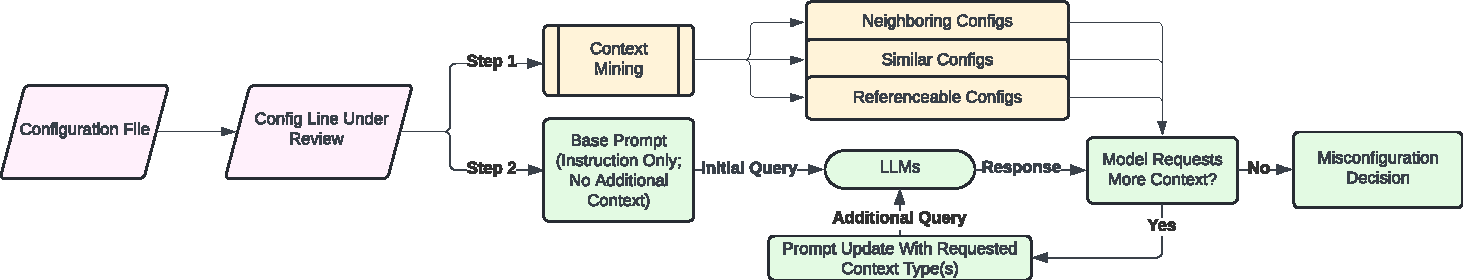
\includegraphics[width=\linewidth]{figs/cap.pdf}
    \caption{\sysname{} system overview.}
    \label{fig:overview}
\end{figure*}

We introduce a tool that tackles the aforementioned challenges via a \emph{context-aware prompting mechanism} (\sysname{}). This approach strategically manages and incorporates only the relevant parts of configurations for each line under review, ensuring that LLMs obtain the required context without succumbing to overload. 
At the same time, this line-by-line methodology provides maximum granularity and emulates the workflow of a human expert, who typically focuses on a single statement to trace its specific dependencies and impacts.
\sysname{} has two components, as
shown in Figure~\ref{fig:overview}:


% \mypara{1. Context Mining:} In this component, \sysname{} mines
% relevant context for a given configuration line under examination. 
% Our definition of relevance extends beyond configurations that are syntactically linked or physically adjacent. \aaron{``Syntactically linked'' seems synonymous with ``referenced policies and objects'' and ``physically adjacent'' seems synonymous with ``neighboring,'' so its odd to say that ``our definition [...] extends beyond [...] syntactically linked or physically adjacent.''} It also includes lines that are \textit{semantically crucial} for a correct interpretation, such as neighboring configurations, similar lines applied in different contexts, or referenced policies and objects that define key parameters.

\mypara{1. Context Mining:} In this component, \sysname{} mines relevant context for a given configuration line under examination. Our definition of relevance is comprehensive, encompassing not only the most direct forms of context—such as physically adjacent (neighboring) lines and syntactically linked (referenceable) policies—but also a more nuanced, \textit{semantically crucial} context: functionally similar lines applied in different parts of the network.

\mypara{2. Guided Prompting:} Once the relevant context has been
mined, the online component engages the LLM through an interactive prompting
process. Instead of overwhelming the model with all the extracted context at
once, \sysname{} interacts with the LLM in a guided manner.

%We now explain the challenges encountered in designing these two components and present the solutions.
We discuss these two components in detail in Sections~\ref{mining_method} and \ref{prompting_method}, respectively.
\section{Context Mining}
\label{mining_method}

The foundation of \sysname{} is its context mining engine. This component is tasked with systematically identifying and extracting information that may be relevant to analyzing a specific line of configuration. The core challenge lies in the complex nature of `relevance' itself, which is not defined by mere proximity in a file. As discussed in Section~\ref{sec:motivation}, configurations contain numerous connections within and across devices. 
% Therefore, to emulate an expert's intuition and capture the full picture of a configuration's correctness—including its local interactions, \aaron{What are ``local interactions?''} network-wide patterns, and distant dependencies—we design a mining process that is guided by configurations' hierarchical structure, relative uniformity~\cite{le2006minerals, kakarla2020finding}, and abundance of references~\cite{benson2009complexitymetrics}.
Therefore, to emulate an expert's intuition, we design a mining process guided by configurations' hierarchical structure, relative uniformity~\cite{le2006minerals, kakarla2020finding}, and abundance of references~\cite{benson2009complexitymetrics} in order to capture the full picture of a configuration's correctness by revealing its local interactions (\ie, how settings within a single block define its behavior), its adherence to network-wide patterns (the implicit design templates), and its distant dependencies (the explicit links between a statement and its definition elsewhere).


\subsection{Representing configurations}
\label{sec:mining_method:structure}

%\begin{wrapfigure}{r}{0.5\columnwidth}
%    \centering
%    \fbox{
\includegraphics[width=0.48\columnwidth]{figs/tree_form.png}}
%    \caption{Example snippet of tree-formatted Juniper router configuration file. \aaron{Groups are a Juniper-specific feature; can we show a snippet of the configuration that is more common across vendors (e.g., interfaces, routing protocols, filters)?}}
%    \label{fig:tree}
%\end{wrapfigure}

Since configurations have a structured, hierarchical format (discussed in Section~\ref{sec:motivation}), we represent each device's configuration as a tree ($T$).
%Configurations are typically written in a structured, hierarchical format that can be effectively modeled as a tree (\(T\)), as shown in the example in Figure~\ref{fig:tree}. 
Each node (\(V\)) corresponds to a specific 
%configuration element, with child nodes providing further specificity.
category (\eg, `{\tt interfaces}', `{\tt filter}'), instance (\eg, `{\tt ge-1/0/1}', `{\tt EXAMPLE-FILTER}'), or parameter (\eg, `{\tt mtu}', `{\tt input}') within the configuration.
%and edges convey the nesting of 
%represent the relationships/dependencies between
%these elements.
A complete path \(
P = \{ \top \rightarrow V_1 \rightarrow V_2 \rightarrow \dots \rightarrow V_k = v_k \}
\) from the root ($\top$) to a leaf ($V_k$) represents a single, \textit{fully-qualified configuration statement} (FQCS). For example, the path listed at the top of Figure~\ref{fig:context_mine} corresponds to line 7 in Figure~\ref{fig:example_config}, where the leaf node ($V_k = v_k$) represents the configuration parameter (`{\tt input}') and its associated value (`{\tt EXAMPLE-FILTER}'), and the preceding nodes ($V_1, V_2, \dots, V_{k-1}$) represent the configuration sections the parameter is nested within (`{\tt interfaces}', `{\tt ge-0/0/1}', ..., `{\tt filter}').

%Let any unique path \(
%P = \{ \top \rightarrow V_1 \rightarrow V_2 \rightarrow \dots \rightarrow V_k = v_k \}
%\) in this tree have \(k\) nodes. The root node (\(\top\)) represents the entry point of the configuration file. The immediate following node (\(V_1\)) corresponds to the broadest configuration category in this path. Intermediate nodes (\( V_2, \dots, V_{k-1} \)) represent increasingly nested configuration sections. Finally, the leaf node \(V_k\) represents a configurable parameter with its associated value \(v_k\). A complete path from the root to a leaf therefore represents a single, \textit{fully-qualified configuration statement} (FQCS), which may be composed of multiple hierarchical lines in the raw text (\eg, the setting `allowed vlans 123` is found within the `interface GE1/1` stanza). %


%\subsection{Contextual Relevance from Different Aspects:} 
\subsection{Principal configuration contexts} 
Based on the characteristics of configurations discussed in Section~\ref{sec:motivation}, we identify three principal forms of context to extract from configurations: (1) neighboring configuration, (2) similar configuration, and (3) referenced configuration.
We define each type of context relative to a specific FQCS ($P = \{ \top \rightarrow V_1 \rightarrow \dots \rightarrow V_k = v_k \}$) under review. As demonstrated by the examples in Figure~\ref{fig:context_mine}, each type of context provides unique insights that contribute to the evaluation of a FQCS. 


% \begin{figure*}[t]
%     \centering
%     \begin{mdframed}
%     \begin{minipage}{0.5\textwidth}
%     \footnotesize % Dynamically scales down font
%     \mypara{Example: Context Mining for a Specific Configuration Line}
    
%     \textit{Configuration Line Under Review:}
%     \begin{Verbatim}
% groups -> INTERFACE-BACKBONE -> interfaces -> <ge-*> -> unit <*>
% -> family inet -> filter -> input-list = "inet-sample"
%     \end{Verbatim}
%     \hrulefill

%     \mypara{Extracted Neighboring Configurations}
%     \begin{Verbatim}
% (a) groups -> INTERFACE-BACKBONE -> interfaces -> <ge-*> -> unit <*>
%     -> family inet -> filter -> input-list = "backbone-in"
% (b) groups -> INTERFACE-BACKBONE -> interfaces -> <ge-*> -> unit <*>
%     -> family inet -> filter -> output = "interface-out"
%     \end{Verbatim}

%     \mypara{Extracted Similar Configurations}
%     \begin{Verbatim}
% (a) groups -> INTERFACE-BACKBONE -> interfaces -> <ge-*> -> unit <*>
%     -> family mpls -> filter -> input-list = "mpls-sample"
%     \end{Verbatim}

%     \mypara{Extracted Referenced Configurations}

%     \mysubpara{(1) Intra-Device Reference}
%     \begin{Verbatim}
% (a) groups -> firewall -> family inet -> filter inet-sample -> term default
%     -> then = sample
% (b) groups -> firewall -> family inet -> filter inet-sample -> term default
%     -> then = next term
%     \end{Verbatim}

%     \mysubpara{(2) Cross-Device Reference}
%     \textit{New Example Line Under Review (on Router A, IP 10.1.2.2):}
%     \begin{Verbatim}
% protocols -> bgp -> group "PEERS" -> neighbor 10.1.2.3 -> description = "to-router-B"
%     \end{Verbatim}
%     \textit{Extracted Context (from Router B's configuration file):}
%     \begin{Verbatim}
% (a) protocols -> bgp -> group "PEERS" -> neighbor 10.1.2.2 -> description = "to-router-A"
%     \end{Verbatim}
%     \end{minipage}
%     \end{mdframed}

%     \caption{An illustration of the four types of context mined by \sysname{} for a given configuration line. The system extracts neighboring, similar, and both intra- and cross-device referenced configurations. \aaron{This needs to be updated to match the example configuration in Figure~\ref{fig:example_config}.}}
%     \label{fig:context_mine}
% \end{figure*}


\begin{figure*}[t]
    \centering
    \begin{mdframed}
    \begin{minipage}{0.95\textwidth} % Using a slightly wider minipage for clarity
    \footnotesize % Dynamically scales down font
    
    \mypara{Example: Context Mining Based on Figure~\ref{fig:example_config}}
    
    \vspace{1em}
    \textit{Configuration Line Under Review (from line 7):}
    \begin{Verbatim}
interfaces -> ge-0/0/1 -> unit 0 -> family inet -> filter -> input = "EXAMPLE-FILTER"
    \end{Verbatim}
    \hrulefill

    \mypara{Extracted Neighboring Configurations}
    \textit{(Other settings for the same interface unit)}
    \begin{Verbatim}
(a) interfaces -> ge-0/0/1 -> unit 0 -> family inet -> address = "10.0.1.1/24"
    \end{Verbatim}

    \mypara{Extracted Similar Configurations}
    \textit{(The same parameter used on a different, but similar, interface)}
    \begin{Verbatim}
(a) interfaces -> ge-0/0/2 -> unit 0 -> family inet -> filter -> input = "EXAMPLE-FILTER"
    \end{Verbatim}

    \mypara{Extracted Referenced Configurations}

    \mysubpara{(1) Intra-Device Reference}
    \textit{(Finding the definition of the referenced "EXAMPLE-FILTER")}
    \begin{Verbatim}
(a) firewall -> family inet -> filter EXAMPLE-FILTER -> term ALLOW-INTERNAL 
    -> from -> source-address = "10.0.0.0/16"
(b) firewall -> family inet -> filter EXAMPLE-FILTER -> term ALLOW-INTERNAL 
    -> then -> accept
    \end{Verbatim}

    \mysubpara{(2) Cross-Device Reference}
    \textit{(New Example Line Under Review (from line 24) on Router A (10.0.2.1)):}
    \begin{Verbatim}
protocols -> bgp -> group "EBGP-PEER" -> neighbor = "10.0.2.2"
    \end{Verbatim}
    \textit{Extracted Context (from peer Router B's configuration file):}
    \begin{Verbatim}
(a) protocols -> bgp -> group "EBGP-PEER" -> neighbor = "10.0.2.1"
    \end{Verbatim}
    
    \end{minipage}
    \end{mdframed}

    \caption{An illustration of the types of context mined by \sysname{}, with concrete examples drawn from the sample configuration in Figure~\ref{fig:example_config}. The system extracts neighboring, similar, and both intra- and cross-device referenced configurations.}
    \label{fig:context_mine}
\end{figure*}

\mypara{Neighboring configurations ($N_m(P)$):}
% Neighboring configurations are lines that are structurally close to the FQCS under review, typically within the same functional block. They provide immediate, local context, revealing potential dependencies or conflicts. \aaron{It's a little confusing to talk about dependencies and conflicts here, because dependencies seems more connected to referenced configurations and conflicts seems more connected to similar configurations. Is there another way we can motivate neighboring configurations?} For instance, when analyzing an IP address on an interface, other settings for that same interface (like its MTU or ACLs) are crucial neighboring context.
Neighboring configurations are lines that are structurally close to the FQCS under review, typically within the same functional block. They provide the immediate, local context necessary to understand the holistic state and intended behavior of a specific entity, such as an interface or routing protocol. For instance, when analyzing an IP address on an interface, its neighboring context—such as whether the interface is administratively shut down, its assigned MTU, or the access lists applied to it—is crucial for correctly interpreting the operational impact of that IP address.


Formally, we define neighboring configurations as the set of paths $P'$ that share a common ancestry with $P$ up to a certain depth, $m$. Let $V_i(P)$ be the $i$-th node in path $P$. The set of neighboring paths is:
\[
N_m(P) = \{ P' \in T \mid V_i(P') = V_i(P) \text{ for } 1 \le i \le m, \text{ and } P' \neq P \}
\]
%This corrected definition ensures the shared nodes are identical. 

The depth parameter $m$ controls the scope of the context. A larger $m$ results in a tighter, more relevant neighborhood.
%\textit{Design Justification:} 
A simple and effective choice is to set $m = k-1$, meaning we extract all sibling configurations that share the same direct parent. This captures the most immediate context without including potentially irrelevant data from higher up in the hierarchy. While we use this default for our evaluation, we acknowledge that a full study on the impact of different values of $m$ is a valuable area for future work.

\mypara{Similar configurations ($S(P)$):}
Similar configurations involve the same type of parameter but applied in slightly different contexts (\eg, the MTU settings on all other interfaces across the network). Comparing these helps detect inconsistencies or deviations from standard practices---which, as discussed in Section~\ref{sec:motivation:llms}, may or may not be intentional.

% Formally, we define similar configurations as the set of paths $P'$ that share the same broadest category node ($V_1$) and the same final parameter node ($V_k$), but differ in their intermediate nodes.
% \[
% S(P) = \{ P' \in T \mid V_1(P')=V_1(P), V_k(P')=V_k(P), P' \neq P \}
% \]
% For example, this allows us to find all `MTU' settings ($V_k$) under the `interfaces' category ($V_1$) across the entire device.

% We require a match up to the $V_1$ node because it typically represents a major functional block (like `interfaces' or `routing-policies'). This provides a meaningful balance; matching only on the root node ($\top$) would be too broad, while requiring deeper matches (like $V_2$) would be too restrictive and might miss relevant comparisons across different sub-sections. \aaron{Should we include an example of why these alternatives would be too broad or restrictive: e.g., finding similar uses of the `action' parameter under $\top$ would include both route filters and packet filters, while matching by a specific interface would find no similar configurations?} \aaron{Should we include a depth parameter in $S(P)$ similar to $N_m(P)$? As a motivating example: `routing' is a $V_1$ node in Juniper router configurations, with specific protocols (`bgp`, `ospf`) as $V_2$ nodes;  it seems odd to compare BGP settings with OSPF settings, which occur when only matching on $V_1$. At the same time, it is unlikely that there will be overlap in $V_K$ between BGP and OSPF settings, so maybe this flexibility is irrelevant. Should we be conducting some empirical analysis of configuration languages to motivate the choice of matching only on $V_1$?}


To provide flexibility, we define similar configurations using a shared ancestry depth, $m$, similar to our approach for neighboring configurations. Formally, we define the set of similar paths as those that share the same ancestry up to depth $m$ and terminate with the same parameter node ($V_k$), but differ in the path between $m$ and $k$.
\[
S_m(P) = \{ P' \in T \mid V_i(P')=V_i(P) \text{ for } 1 \le i \le m, V_k(P')=V_k(P), \text{ and } P' \neq P \}
\]

The choice of the depth parameter $m$ allows for a crucial trade-off between the breadth and relevance of the comparison. Our default choice is to set $m=1$, which typically represents a major functional block (like `interfaces' or `protocols'). This provides a meaningful balance, which can be illustrated by considering the alternatives:
\begin{itemize}
    \item A choice of $m=0$ (matching only on the root node $\top$) would be too broad. For example, searching for a parameter like `action' would incorrectly group together firewall filter actions and route policy actions, which are semantically very different.
    \item A choice of $m$ that is too high (\eg, $m = k-2$, matching on a specific interface like `ge-0/0/1') would be too restrictive. A search for similar MTU settings would find no configurations on other interfaces, defeating the purpose of the comparison.
\end{itemize}

The flexibility of $m$ also helps manage comparisons within large functional blocks. For instance, in a Juniper configuration, `protocols' is a $V_1$ node containing specific protocols like `bgp' and `ospf' as $V_2$ nodes. Our default of $m=1$ would compare settings across BGP and OSPF. This may seem odd, but in practice, the final parameter names ($V_k$) are typically distinct between protocols, so irrelevant comparisons are rare. However, for a more targeted analysis, a user could set $m=2$ to find similar settings only within BGP or within OSPF. While our default provides a reasonable starting point, to suit different analysis cases, \sysname{} supports the flexibility to choose optimal default values for $m$ for different parameter types.



\mypara{Referenced Configurations (Intra- and Cross-Device):}
Referenced configurations provide the definitions for user-defined identifiers --- custom labels created by an administrator to name a specific object or policy, such as an access-list name, a policy-map, or a BGP peer group. Referenced configurations are the stanzas that provide the actual definitions for these identifiers. Mining this context is crucial for understanding dependencies, but the nature of these references can be either internal to a single device's configuration or external, pointing to another device on the network. \sysname{} is designed to handle both.

\mysubpara{1. Intra-Device Referencing:}
This is the most common form, where a value in one part of a configuration refers to a policy or object defined elsewhere in the same file. For example, a line like `import-policy = PolicyX` is a reference. To resolve this, the context mining engine searches for the stanza where `PolicyX` is defined, such as the `policy-options $\rightarrow$ policy-statement PolicyX $\rightarrow$ ...' block, which contains the actual rules for that policy.

Formally, for a given path $P$ in a device's configuration tree $T$, we define this set of intra-device references, $R_{intra}(P)$, as the set of paths $P'$ where the value of the original path, $v_k(P)$, appears as an intermediate node.
\[
R_{intra}(P) = \{ P' \in T \mid P' =  \top \rightarrow \dots \rightarrow v_k(P) \rightarrow \dots \rightarrow V_j = v_j \}
\]
Here, $v_k(P)$ is no longer a leaf node but part of the path in $P'$, indicating that it is being defined or elaborated upon.


% \mypara{Differentiating Pre-defined Keywords from User-defined Identifiers:} \aaron{Still need to refine and integrate this part}

A primary challenge in extracting intra-device referenceable configurations is the risk of incorporating irrelevant context. This risk stems from the difficulty of distinguishing between \textit{pre-defined parameter values} and \textit{custom user-defined parameter values}.
Pre-defined keywords are part of the vendor's standard configuration language and have a fixed, universal meaning (\eg, the boolean values `true' and `false', interface modes like `trunk' or `access', or protocol names like `any' or `ospf'). In contrast, user-defined identifiers are custom labels created by an administrator to name a specific object or policy (\eg, a policy map name like `QOS-VOIP-POLICY', an access list name such as `BLOCK\_GUEST\_ACCESS', or a VLAN ID like `1000'). This distinction is critical because it dictates our context-mining strategy: a user-defined identifier acts as a pointer, implying that its full definition exists elsewhere in the configuration and \textit{must} be retrieved. 
Misidentifying a custom policy name as a pre-defined keyword would prevent the system from searching for its essential definition, likely causing it to miss critical dependency-related errors. Conversely, mistakenly treating a standard keyword like `true' as user-defined would trigger a pointless and computationally expensive search for a non-existent or mismatched definition.



To solve this, we initially considered a simple heuristic based on existence checks in the configuration's hierarchical tree structure. This method assumed that any parameter value that also appeared as a parent or intermediate node elsewhere in the configuration must be user-defined. However, this approach proved brittle, as it could be fooled by coincidences in naming and lacked a true understanding of the configuration's grammar. We then explored a more advanced majority-voting mechanism, which attempted to enforce consistency by assuming that a given parameter type (like `timeout') should always take the same class of value (pre-defined or user-defined). This, too, had a critical flaw: it could not distinguish between identical parameter values used in different contexts. For example, it would struggle to differentiate between the user-defined `vlan-id 1000' and the user-defined `access-list 1000', as it would incorrectly try to enforce a uniform classification on the value `1000' based on its other uses, imposing a false consistency.


Therefore, \sysname{}'s final design discards these rule-based heuristics in favor of a more direct and robust \textit{LLM-based approach}. As part of its initial query, our framework explicitly instructs the LLM to classify the value not in isolation, but \textit{in the context of the full configuration line it appears in}. By leveraging its vast training on vendor-specific documentation and millions of real-world configuration examples, the LLM has learned the expected syntax and value patterns for different configuration parameters. It understands that the value following a parameter like `vlan-id' is a user-created label, while the value following a command like `ip routing' is a pre-defined boolean keyword. This allows it to easily and accurately determine that `1000' is a distinct, user-defined identifier in the context of a VLAN versus an ACL, correctly handling the ambiguity that plagued the previous methods. This approach requires no complex, hand-crafted rules and has proven to be significantly more accurate and reliable.

\mysubpara{2. Cross-Device Referencing:}
A more complex challenge arises when a user-defined identifier refers to another device on the network. This is common in configurations for routing protocols, VPNs, or services. For example, in a BGP configuration, the line `neighbor 10.1.1.2 remote-as 65001' contains an identifier, `10.1.1.2', for a peer router. The most critical context for verifying this line is not on the current device, but on the device at `10.1.1.2'.

Our methodology for this is a three-step process:
\begin{enumerate}
    \item \textbf{Identify External Reference:} The system first identifies that a value (like an IP address or hostname) is an identifier for an external device.
    \item \textbf{Locate Target Device:} It then looks up the corresponding configuration file for that target device from our set of network-wide configurations.
    \item \textbf{Find Reciprocal Configuration:} Finally, it searches within the target device's configuration for lines that reference the \textit{original} device back. For the BGP example, if our original device's IP is `10.1.1.1`, the system would search the configuration of `10.1.1.2` for the corresponding `neighbor 10.1.1.1 ...` statement.
\end{enumerate}

Formally, let the current device's configuration tree be $T_A$ and its network identifier be $id(T_A)$. If the value $v_k(P)$ in a path $P \in T_A$ is an identifier for another device with configuration tree $T_B$, the set of cross-device references, $R_{cross}(P)$, is defined as:
\[
R_{cross}(P) = \{ P' \in T_B \mid id(T_A) \in P' \}
\]
This captures all configuration statements on the target device that mention the original device. This process is essential for verifying connectivity and detecting symmetric misconfigurations where, for example, a session is configured on one side but not the other.
The complete set of referenced configurations, $R(P)$, encompasses both intra-device definitions found within the same configuration file and cross-device configurations located on a target device that refer back to the original device.

\mypara{Composable Context Primitives:}
It is important to note that the three principal context types---Neighboring, Similar, and Referenced---serve as atomic building blocks, or \textit{primitives}. A key strength of our framework is the ability to compose these primitives to form more complex and powerful context queries. For example, we can compose S(R(P)), which translates to finding configurations that are \textit{similar} to the \textit{definition} of a value in the line under review. Conversely, a composition of R(S(P)) would find the \textit{definitions} of values that appear in \textit{similar} configurations. This compositional nature, which also allows for queries like R(N(P)) (the definitions of values in neighboring lines), gives \sysname{} the flexibility to emulate the multi-step, intuitive reasoning of a human expert.
\section{Iterative Prompting}
\label{prompting_method}

As we transition from context mining to utilizing the extracted information in LLM prompts, the next challenge is how to feed this information into the model without overwhelming it. While extracting accurate and relevant context is essential, the model's ability to process that information effectively is just as crucial.

% A significant limitation of many LLM-based approaches is context overload, where the model is fed too much information at once, causing it to lose focus on the most pertinent details. This is especially relevant in network configurations, where dependencies and relationships between different configuration lines can be complex and spread throughout the file.




\mypara{Solution:}
To address these issues, \sysname{} implements an iterative, sequential prompting framework that allows the model to request and process relevant context in stages. Instead of overwhelming the model with all available context at once, \sysname{} enables the model to actively request additional information as needed. This approach enhances the model’s ability to maintain focus, coherence, and overall detection accuracy by allowing it to prioritize and process context more effectively, ensuring that only the most pertinent information is presented at each step.

\mysubpara{1. Initial Prompting:} The process begins by feeding the LLM the specific configuration line under review, along with targeted instructions about the type of misconfiguration we are checking for (\eg, syntax errors, dependency conflicts, or just general misconfiguration).
% This prompt is concise, providing only the critical line and the request as shown in the example in 
Figure~\ref{fig:initial_prompt} presents an example where the initial prompt
includes MTU configuration line with an instruction to identify any
syntax misconfigurations related to that configuration.
This reduces the initial information load and allows the model to focus on the core issue.
\aaron{Update this to reflect most recent prompting}

    \begin{figure}[tb]
    \centering
    \fbox{
\includegraphics[width=0.95\columnwidth]{figs/initial_prompt_response.png}}
    \caption{Example: initial prompting and LLM context request response for detecting syntax misconfiguration.}
    \label{fig:initial_prompt}
\end{figure}

\mysubpara{2. Contextual Options:} Next, \sysname{} offers the model the option to request additional context based on its understanding of the configuration line and the misconfiguration detection request. These options are based on our categorized context types, including: neighboring (\( N(P) \)), similar (\(S(P) \)) , and referenceable contexts (\( R(P) \)), as well as referenceable contexts on neighboring configurations (\( N(R(P)) \)) \aaron{Formalism seems inverted from description}. By allowing the model to choose which context to receive, \sysname{} ensures that the LLM is only given information that is most relevant to the detection task at hand, reducing the risk of context overload. Figure~\ref{fig:initial_prompt} illustrates an example request response
where the LLM requests neighboring context and referenceable contexts on neighboring configurations after the initial prompt to aid analyzing the MTU setting.
    
\mysubpara{3. Iterative Refinement:} After the model processes the initial prompt, it can request additional information if needed before arriving at the final decision. \aaron{How often is additional (i.e., a second round of) context requested?} \sysname{} engages in a feedback loop where the model’s output informs the next set of prompts. For instance, if the model identifies a possible syntax issue but requires more context from a related policy definition, \ie, similar context, \sysname{} can deliver that specific context in the next prompt. This iterative process continues until the model has sufficient information to make a well-informed decision. Figure~\ref{fig:feedback_and_response} provides an example of what a final misconfiguration decision looks like regarding a misconfiguared MTU value.
    \begin{figure}[tb]
    \centering
    \fbox{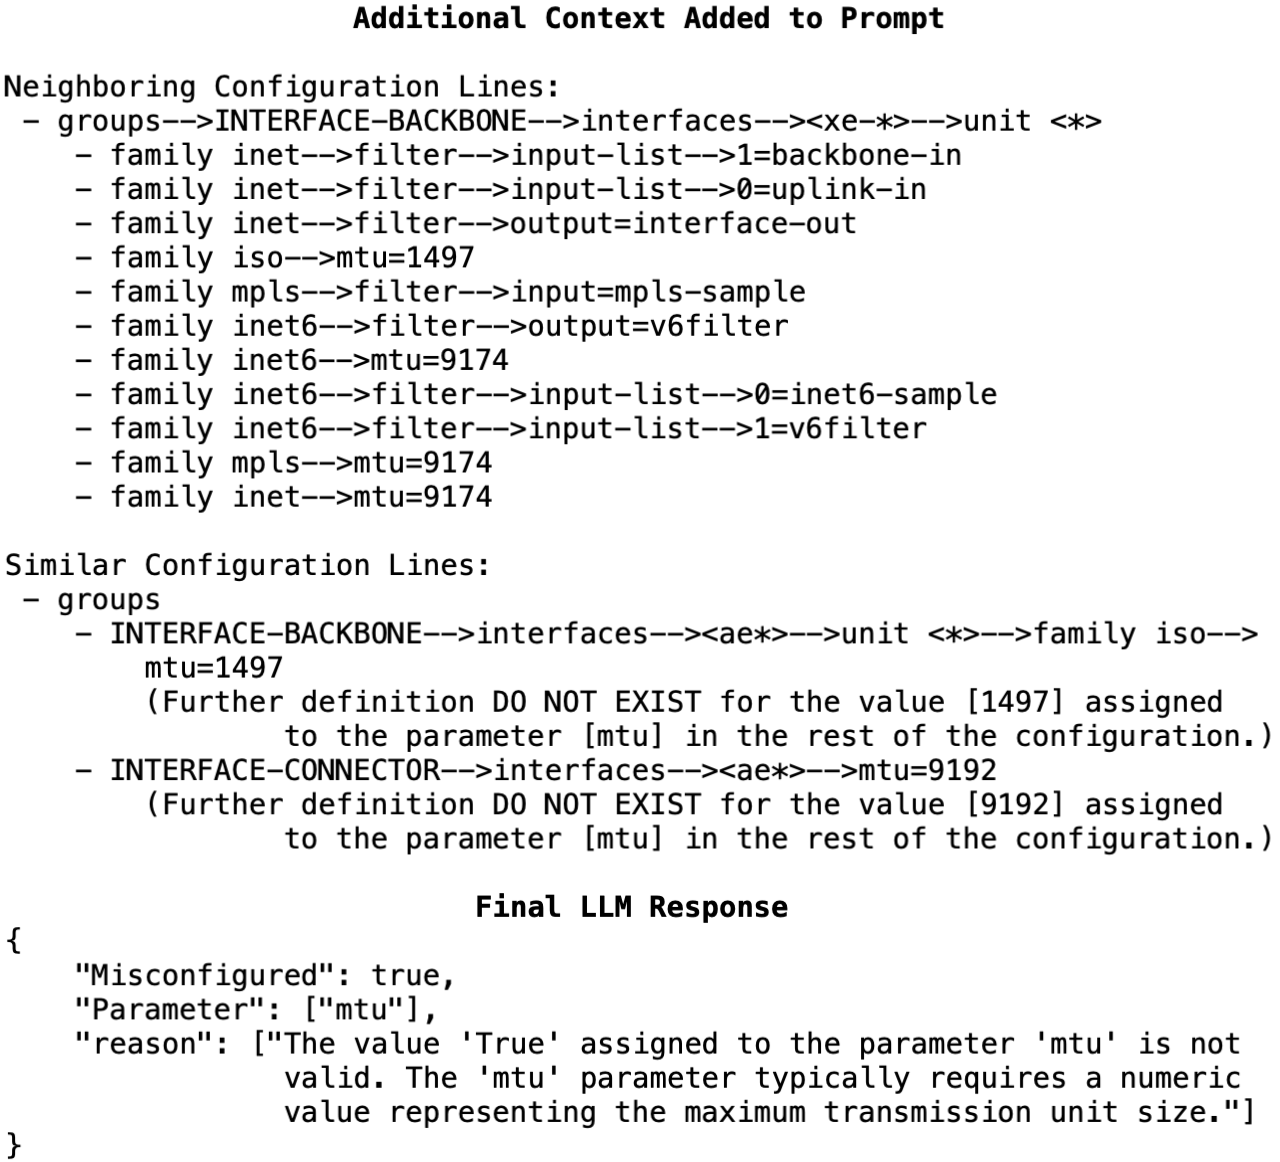
\includegraphics[width=0.95\columnwidth]{figs/feedback_and_response.png}}
    \caption{Example: Adding requested context and retrieving misconfiguration detection result.}
    \label{fig:feedback_and_response}
\end{figure}


This sequential, interactive approach mirrors how a network administrator might manually review a configuration file—examining the most relevant sections first, then digging deeper into referenceable or adjacent configurations as needed.

% It ensures that the model focuses on the most critical aspects of the configuration without becoming overwhelmed by extraneous information.

\mypara{Why Iterative, Requested Based Prompting Works:}
By breaking down the context into smaller, more digestible portions, \sysname{} addresses the fundamental challenges of context overload. This method significantly enhances the model’s ability to:
\begin{enumerate}
    \item Stay on target: With less irrelevant information, the model can maintain focus on the specific issue under review.
    \item Preserve coherence: Incrementally adding information allows the model to build a more coherent understanding of the configuration~\cite{li2023prompt,subramonyam2024bridging}, improving detection of complex issues such as dependency conflicts or misapplied policies.
    \item Optimize performance: Avoiding context overload reduces the processing burden on the model, leading to faster and more reliable outputs.
\end{enumerate}

For example, in detecting misconfigurations in a multi-layer firewall policy, \sysname{} might first present the core rule in question, then iteratively offer neighboring rules that affect the same traffic flow, followed by referenceable configuration sections that define broader network policies. This structured process ensures that the LLM has all the information it needs, without drowning in unnecessary details, enabling it to make accurate decisions. Unlike conventional prompt-chaining, which provides incremental instructions based on a fixed context, \sysname{} dynamically adds context as requested by the LLM, focusing on the evolving needs of the analysis.

% By combining efficient context extraction with iterative, focused interaction, \sysname{} represents a significant advancement in leveraging LLMs for router misconfiguration detection, ensuring that models are both effective and computationally efficient.

\section{Evaluation}
\label{sec:eval}
To evaluate the effectiveness of \sysname{}, we assess its performance across a range of real-world and synthetic network configurations. Our evaluation is structured around four key research questions:
%, which allow us to examine \sysname{}'s capabilities under both targeted and open-ended conditions and to compare its behavior against state-of-the-art detection methods.

%The evaluation will address the following questions in order:
\begin{enumerate}
    \item Can \sysname{} accurately detect known misconfigurations in controlled and real-world settings?
    \item Can \sysname{} identify novel, previously unknown issues in large-scale networks?
    \item What types of contextual information do different Large Language Models (LLMs) request when diagnosing issues, and how does this affect their performance?
    \item How does \sysname{}'s detection capability compare to existing state-of-the-art verification tools?
\end{enumerate}

%We now describe the datasets and experimental setup used to address these questions, followed by detailed findings in the subsequent sections.

\subsection{Evaluation Setup}

\mypara{Datasets:}
Our evaluation uses three distinct sets of network configurations obtained from a nationwide Research \& Education Network (Internet2), a medium-scale campus network (Campus A), and a large-scale campus network (Campus B). We sample representative routers from each environment for evaluation. Table~\ref{tab:dataset_summary} provides an overview of these datasets.



\begin{table}[t]
\centering
\resizebox{\columnwidth}{!}{
\begin{tabular}{|l|l|c|l|r|r|}
\hline
\multirow{2}{*}{\textbf{Dataset}} & \multirow{2}{*}{\textbf{Vendor(s)}} & \textbf{No. Devices} & \multirow{2}{*}{\textbf{Device Roles}} & \multicolumn{2}{c|}{\textbf{Avg. Config Length}} \\
\cline{5-6}
& & \textbf{Sampled} & & \textbf{Lines} & \textbf{Tokens} \\ \hline
Internet2 & Juniper & 17 & TBA & ~18,944 &  \\
Campus A & Aruba & 8 & TBA & ~5,563 & \\
Campus B & Cisco, Juniper & 5 & Distribution \& Aggregation Routers & ~6,261 & \\ \hline
\end{tabular}
}
\caption{Overview of Network Configurations Used in Evaluation.}
\label{tab:dataset_summary}
\end{table}

\mypara{Context Extraction Hardware:}
The machine we use for context extraction has a single AMD EPYC 7302P (3GHz, 16-Core/32-Thread, 128MB L3 cache) processor and 64GB of memory. We do not use GPU acceleration, because \sysname{}'s context extraction and orchestration logic is CPU-parallelizable and does not significantly benefit from the GPU.

\mypara{Querying LLMs:}
We evaluate \sysname{} using GPT-4o~\cite{achiam2023gpt}
%OpenAI's latest model optimized for complex reasoning and long-context tasks 
(context window: 128,000 tokens; max output: 4,096 tokens; training cutoff: October 2023)
and DeepSeek-V3 (DS)~\cite{deepseekai2024deepseekv3technicalreport}
%DeepSeek-AI's open-source transformer suited for structured code and configuration analysis
(context window: 128,000 tokens; max output: 8,000 tokens; training cutoff: July 2024). For all experiments, we use the official chat completions APIs. This API is inherently stateless, which is critical for reproducibility, as each call is an independent event. To enable our iterative diagnostic process, our framework simulates a stateful conversation by constructing a complete, ordered history for each new query. Specifically, every API call includes the full sequence of prior prompts, the model's requests for context, the context provided by \sysname{}, and the model's intermediate reasoning steps. This method provides the best of both worlds: the controlled, reproducible environment of a stateless API, and the sophisticated, multi-step reasoning of a stateful dialogue, with our framework maintaining full control over the conversational history at every step.

\subsection{Can \sysname{} Detect Known Misconfigurations?}

We first evaluate \sysname{}'s effectiveness in detecting misconfigurations with a known ground truth. This is a crucial baseline for establishing accuracy. We conduct this analysis in two distinct settings: first, using synthetically generated but realistic errors injected into production configurations from Internet2, and second, using real, known misconfigurations from the Campus A network.

\mypara{Detecting Synthetic Misconfigurations in Internet2:}
To create a controlled environment for measuring detection performance, we obtained snapshot configurations from Internet2 (Juniper devices) and introduced 32 updates, comprising 16 correct updates (the original lines of config) and 16 erroneous modifications. These errors, inspired by misconfigurations identified in prior work~\cite{some_prior_work}, are categorized into three types:

\begin{itemize}
    \item \textit{Syntax errors} occur when the configuration does not adhere to the expected format or structure---\eg, a missing bracket or misused keyword in a BGP routing policy.
    \item \textit{Range violations} involve parameter values that fall outside the acceptable range---\eg, an MTU value that exceeds the maximum allowed for a specific interface type.
    \item \textit{Dependency/conflict (D/C) issues} arise when different configuration lines are incompatible or contradict each other. This broad category covers both dependency errors (\eg, a reference to a non-existent group) and consistency/conflict errors (\eg, a firewall rule that blocks traffic another policy explicitly permits).
\end{itemize}

For syntax and range errors, we created four distinct misconfigurations each. For D/C misconfigurations, we introduced eight distinct errors, as vanilla LLMs often excel at detecting localized syntax and range issues, while \sysname{}’s context mining is particularly effective for uncovering nuanced D/C issues that require broader understanding. The additional D/C errors allow us to thoroughly assess this core capability. Table~\ref{tab:syn_configs} provides details on these errors. Note that some errors involve Juniper's `apply-groups` feature, a unique mechanism for configuration inheritance that can challenge tools not specifically designed to reason about it.

For this case study, the \sysname{} implementation is powered by \textbf{GPT-4o}. For each update, we run \sysname{} by treating the modified line as the line under review and conducting the iterative prompting process. 
%Based on our finding that asking the model to search for `GENERAL` misconfigurations led to successful detection, we used this simpler, more general prompt for the analysis, rather than prompting for specific error types individually. 
To provide qualitative insight into the detection process, Table~\ref{tab:syn_responses} in Appendix~\ref{subsec:example_llm_reasoning} shows representative examples of the reasoning provided by the LLM when identifying several of the misconfigurations.



The results of this case study demonstrate the effectiveness of our iterative, context-aware approach. \sysname{} successfully identified all 16 synthetic misconfigurations while correctly validating all 16 correct updates, achieving 100\% accuracy with zero false positives or false negatives.
The analysis of the requested context in Table~\ref{tab:syn_configs} reveals a key insight into this success. For simple, self-contained syntax errors like a missing brace, the LLM correctly determined that no additional context was needed to identify the issue. However, for more complex range and D/C errors, the model consistently requested the precise contextual information required for a correct diagnosis. For instance, to validate a prefix limit (`Range' error) or a policy (`D/C' error), it asked for definitions and similar lines (R(P) and S(P)). This confirms that the two-step process—where the model first identifies and requests necessary evidence before making a final judgment—is critical for achieving high accuracy on nuanced configuration errors that are impossible to detect from a single line in isolation.

\begin{table}[tb]
\centering
\resizebox{\columnwidth}{!}{
\begin{tabular}{|l|l|l|l|}
\hline
\textbf{Type} & \textbf{Description} & \textbf{Misconfig Example} & \textbf{Requested Context}\\ \hline

\multirow{4}{*}{\textbf{Syntax}} 
& Missing closing brace &...interfaces: \{\textcolor{red}{"<ge-*"}: & None\\ \cline{2-4}
& Invalid keyword for value & ...mtu: \textcolor{red}{"True"}    & \( N(P) \), \( R(P) \)\\ \cline{2-4}
& Incorrect hierarchical placement & ...host-name: \textcolor{red}{"\{rtsw.alba-re1\}"}  & \( N(P) \)\\ \cline{2-4}
& Invalid IP address format & ...neighbor: \textcolor{red}{192.168.253.1.1}" & \( N(P) \), \( R(P) \)\\ \hline

\multirow{4}{*}{\textbf{Range}}  
& MTU exceeds interface max & ...mtu: \textcolor{red}{"10000"}  & \( N(P) \), \( R(P) \)\\ \cline{2-4}
& VLAN ID outside standard 1-4094 range & ...vlan-id: \textcolor{red}{"5000"}  & \( N(P) \), \( R(P) \), \( R(N(P)) \) \\ \cline{2-4}
& AS number outside valid range & ...autonomous-system: \textcolor{red}{70000} & \( N(P) \), \( R(P) \) \\ \cline{2-4}
& Prefix limit exceeds typical values & ...maximum: \textcolor{red}{"200000"} & \( N(P) \), \( R(P) \)  \\ \hline

\multirow{8}{*}{\textbf{D/C}}  
& Reference to a non-existent group & ... apply-groups: \textcolor{red}{"L2-LSP-ATTRIBUTES”} & \( N(P) \), \( R(P) \), \( R(N(P)) \) \\ \cline{2-4}
& Contradictory actions in a policy & ...community \textcolor{red}{add I2CLOUD-EXTENDED-TARGET}  & \( N(P) \), \( R(P) \), \( R(N(P)) \) \\ \cline{2-4}
& Reference to a non-existent filter & ...input-list: \textcolor{red}{"uplink"} & \( N(P) \), \( R(P) \)  \\ \cline{2-4}
& Reference to a non-existent policy & ...export: \textcolor{red}{"OESS-400-300-LOOP} & \( R(P) \)  \\ \cline{2-4}
& Applying an IPv6 filter to MPLS family & ...family mpls: filter:input-list:\textcolor{red}{"v6filter"} & \( R(P), S(P) \)  \\ \cline{2-4}
& Sampling disabled for one protocol family & ...family inet6: \textcolor{red}{SAMPLING MISSING/DISABLED}& \( R(P), N(P) \)  \\ \cline{2-4}
& Mismatch between VRF target and RD & ...vrf-target target:11537:\textcolor{red}{"313001"}& \( S(P) \)  \\ \cline{2-4}
& Unusually small MTU for ISO family & ...family iso: mtu: \textcolor{red}{"1497"}& \( R(P), S(P) \)  \\ \hline
\end{tabular}}
\caption{Erroneous Configuration Updates Introduced and LLM Requested Context for \sysname{}. The descriptions have been clarified to explain the nature of each error.}
\label{tab:syn_configs}
\end{table}



% \begin{table}[ht]
% \centering
% \resizebox{\columnwidth}{!}{
% \begin{tabular}{|l|l|l|p{8cm}|} % Define a fixed width for the Reason column
% \hline
% \textbf{Type} & \textbf{Misconfig} & \textbf{errParameter} & \textbf{Reason}\\ \hline

% \multirow{3}{*}{\textbf{Syntax}} & \multirow{3}{*}{Missing brace} & \multirow{3}{*}{["<ge-*>"]} & "MTU value for 'family inet' is set to 9174 which is less than the interface MTU value of 9192. The MTU for 'family inet' should not be less than the interface MTU."\\\hline

% \multirow{4}{*}{\textbf{Range}} & \multirow{4}{*}{Invalid VLAN ID} & \multirow{3}{*}{["maximum"]} & "The 'maximum' value of 200000 in the configuration line under review significantly exceeds the 'maximum' values of 1000 found in similar configuration lines, indicating a potential range misconfiguration."\\\hline

% \multirow{20}{*}{\textbf{D/C}} & \multirow{5}{*}{Policy Conflict} & \multirow{5}{*}{["remove-comms-rt"]} & "There is a conflict in the configuration under term 'remove-comms-rt' where the action 'community add I2CLOUD-EXTENDED-TARGET' is followed by 'community delete I2CLOUD-EXTENDED-TARGET' which are contradictory actions."\\\cline{2-4}

%  & \multirow{5}{*}{Disabled Sampling} & \multirow{5}{*}{["inet6"]} & "The family mpls is incorrectly using the IPv6 filter inet6-sample v6filter, which is intended for family inet6 in similar configuration lines. MPLS traffic should have its own specific filter, as the filtering requirements for MPLS are different from those for IPv6."\\\cline{2-4}
%  & \multirow{5}{*}{VRF Target Conflict} & \multirow{5}{*}{["target"]} & "The route-distinguisher (RD) in neighoring configurations is set to 11537:381841, while the vrf-target is set to target:11537:313001. These values should typically align, or at least follow certain conventions for mapping VRFs to the correct target instances in MPLS/BGP L2VPN."\\\cline{2-4}
%  & \multirow{5}{*}{Incorrect Filter Usage} & \multirow{5}{*}{["input-list"]} & "The family mpls is incorrectly using the IPv6 filter inet6-sample v6filter, which is intended for family inet6 in similar configuration lines. MPLS traffic should have its own specific filter, as the filtering requirements for MPLS are different from those for IPv6."\\\hline
% \end{tabular}}
% \caption{Example LLM Reasoning for \sysname{}.}
% \label{tab:syn_responses}
% \end{table}

\mypara{Detecting Known Misconfigurations in Campus A:}
To complement the synthetic analysis, we test \sysname{}'s ability to find known, real-world misconfigurations in the Campus A network. The network operators for this campus were specifically interested in detecting incorrect `VLAN assignments'—a type of misconfiguration that often requires a network-wide view, as deviations from uniform configurations across devices can indicate potential issues.
 This scenario demonstrates \sysname{}'s flexibility and we used both the \textbf{GPT-4o} and \textbf{DeepSeek-V3} backends.
 
 % To detect this specific issue, we augmented its default context library with a custom `Inter-Router Consistency Context', which mines the prevalence of a parameter-value pair across all other devices in the network.
 
 % For this analysis, we used both the \textbf{GPT-4o} and \textbf{DeepSeek-V3} backends.

In this targeted analysis, \sysname{} demonstrated perfect accuracy, correctly identifying all 6 known cases of incorrect VLAN assignments (100\% true positive rate). Both LLM backends yielded identical results. Among the six detected cases, two were previously unnoticed yet genuine misconfigurations that had been causing misrouting and network access issues, representing high-severity problems for network operations. The remaining four cases were intentional, benign misconfigurations applied to test and experimental devices.



\subsection{Can \sysname{} Accurately Identify New Issues?}

Beyond detecting known error types, a key goal for \sysname{} is to discover latent or novel misconfigurations in large, complex networks. To evaluate this capability, we performed a comprehensive verification of configuration snapshots from Campus A (Aruba devices) and Campus B (Cisco and Juniper devices). 
%Unlike the previous tests, no update information or error hints were provided. Instead, \sysname{} was instructed to exhaustively analyze full configurations to surface any deviations from general policy correctness and best practices.
In particular, each line of configuration from a subset of devices was fed to \sysname{} to determine if it contained an error.
For each misconfiguration detected by \sysname{}, we verified the correctness of the inference with domain experts from the respective campus networks. 
This open-ended approach allows us to not only assess \sysname{}'s scalability and discovery potential but also to evaluate whether different LLM backends---\textbf{GPT-4o} and \textbf{DeepSeek-V3}---surface distinct issues or exhibit different reasoning patterns. 

\mypara{Campus A: Discovering Genuine Misconfigurations:}
In the analysis of Campus A configurations, \sysname{} successfully detected several previously unknown types of misconfigurations, as shown in Table~\ref{tab:real_results}. The detection results were consistent across both the GPT-4o and DS backends. We categorize the detected misconfigurations by their potential impact on network operations, as determined by the LLM and verified by experts.
% \aaron{These details are already included in Table~\ref{tab:real_results}, so do we need them in the text?}
% \begin{itemize}
%     \item \textit{High Severity}: Misconfigurations in this category pose critical risks to the network and require immediate action. \sysname{} identified invalid subnet mask (\eg, 255.255.253.0) usages that violate binary boundary rules, which could lead to routing issues and network instability.
%     \item \textit{Low Severity}: These issues may not immediately disrupt network operations but should be addressed to ensure optimal functionality and avoid potential risks. \sysname{} identified many instances of misnamed configurations (\eg, `smnpread' instead of `snmpread' for `snmp\_communities') and the inclusion of an insecure SSH key exchange (KEX) algorithm (`diffie-hellman-group14-sha1'), which do not break the system but could lead to confusion and maintenance challenges.
%     \item \textit{Ambiguous}: These misconfigurations are related to configurations that lead to undefined or nondeterministic behaviors. \sysname{} found ambiguous rate limit values (`interval' and `burst' set to 0), which can cause unpredictable performance issues due to missing documentation on how these values should be handled.
% \end{itemize}
Specifically, \sysname{} successfully identified 19 misconfigurations in the Campus A data: two cases of invalid subnet masks, 14 instances of inconsistent policy naming, one insecure SSH KEX algorithm, and two ambiguous rate limit values. Upon validation with domain experts, all 19 cases were confirmed to be either valid misconfigurations or justifiable concerns, resulting in a true positive rate (TPR) of 100\% for this dataset.

\begin{table}[tb]
\centering
\resizebox{\columnwidth}{!}{
\begin{tabular}{|l|l|l|l|}
\hline
{\textbf{Misconfigs}} & {\textbf{Count}} &  {\textbf{Severity (Reason)}} & \makecell{\textbf{True Positive} \\ \textbf{Rate (TPR)}}\\
\hline
%\multirow{2}{*}{\makecell[{{l}}]{Targeted}} &\multirow{2}{*}{\makecell[{{l}}]{Wrong VLAN\\Assignment}} & \multirow{2}{*}{\makecell{6}} & 
%\multirow{2}{*}{\makecell[{{l}}]{\textit{High}: Wrong VLANs permitted in configuration, causing access issues.}} & \multirow{2}{*}{\makecell{6/6 (100\%)}}\\ 
%&&&& \\\hline
\makecell[l]{Invalid subnet\\ mask} & {2} & {\textit{High}: Subnet mask violating binary boundary rules (\eg, 255.255.253.0).}
& \multirow{2}{*}{\makecell{2/2 (100\%)}}\\ 
\hline
 \makecell[l]{Inconsistent \\policy naming} & {14} & {\textit{Low}: Misnamed `smnpread' for `snmp\_communities', but with consistent usage.} & {14/14 (100\%)} \\ 
\hline
\makecell[l]{Insecure SSH \\KEX algorithm} & {1} & {\textit{Low}: Insecure `diffie-hellman-group14-sha1' included in algorithm choices.} & {1/1 (100\%)}\\ 
\hline
\makecell[l]{Ambiguous rate\\limit values} & {2} & {\textit{Ambiguous}: `Interval' and `burst' set to 0, leading to nondeterministic behaviors.} & {2/2 (100\%)} \\ 
\hline
\end{tabular}}
\caption{\sysname{}-detected misconfigurations in comprehensive analysis of Campus A configurations.}
\label{tab:real_results}
\end{table}

\mypara{Campus B: The Challenge of False Positives:}
In contrast to the genuine misconfigurations identified in Campus A, the analysis of the Campus B snapshots highlights the challenge of false positives in open-ended discovery. As detailed in Table~\ref{tab:grouped_misconfig_analysis}, all configurations flagged as potential issues in Campus B were subsequently validated as correct and intentional by network operators. Representative cases of these false positives include:

\begin{itemize}
\item \textit{Duplicate or overlapping DHCP helpers}, which were flagged by the models but were intentionally deployed for redundancy and failover purposes.

\item \textit{Missing VLANs in trunk links} and \textit{Uncoordinated channel-group assignments}, which appeared inconsistent when viewed in isolation but were confirmed to be benign due to compensatory downstream configurations or manual overrides.

\item \textit{Unexpected PIM passive usage}, which aligned with localized multicast policies specific to that campus, albeit being undocumented in standard configuration templates.
\end{itemize}

Interestingly, the two LLM backends showed a significant divergence in behavior on this dataset. GPT-4o consistently classified all 21 instances as misconfigurations, whereas DeepSeek-V3 exhibited more conservative behavior, labeling only a subset as problematic (\eg, it flagged only 4 of the 8 DHCP helper cases and none of the 9 missing VLAN instances). This difference in behavior underscores the importance of model choice and is analyzed further in the next section.

\begin{table}[tb]
\centering
\resizebox{\columnwidth}{!}{
\begin{tabular}{|l|c|l|l|}
\hline
\textbf{Misconfiguration Type (False Positives)} & \textbf{Count} & \textbf{GPT-4o Decision} & \textbf{DeepSeek Decision} \\
\hline
\textit{Duplicate or overlapping DHCP helpers} & 8 & Misconfig (8/8) & 4 Misconfig, 4 No Misconfig \\
\hline
\textit{Missing VLANs in trunk links} & 9 & Misconfig (9/9) & No Misconfig (9/9) \\
\hline
\textit{Uncoordinated channel-group assignment} & 2 & Misconfig (2/2) & No Misconfig (2/2) \\
\hline
\textit{Unexpected PIM passive usage} & 2 & Misconfig (2/2) & No Misconfig (2/2) \\
\hline
\end{tabular}}
\caption{Campus B Non-Targeted Snapshot: All configurations flagged as misconfigurations were later validated by network operators as \textbf{correct} (\ie, \textit{false positives}).}
\label{tab:grouped_misconfig_analysis}
\end{table}

We acknowledge the limitation of not having a definitive true negative or false negative rate for this non-targeted analysis. This is an inherent challenge in evaluating any network verifier on production networks where the complete ground truth of all latent errors is unknown. The analysis of synthetic misconfigurations presented in the previous section, where we observed no false negatives, currently serves as the best available measure in this regard.


\subsection{What Context Do LLMs Request?}
\label{subsec:analysis}

To understand the reasoning behind the models' detection performance—including the causes of the false positives detailed in the previous section—we now analyze the contextual information that each LLM requests within the \sysname{} framework. In \sysname{}, the model itself explicitly selects the context it wants to see from a predefined library. Once requested, the framework faithfully provides the exact lines or definitions without transformation or interpretation.

This design is crucial because it decouples context retrieval from context reasoning. It ensures that downstream decisions—correct or incorrect—are entirely the result of the model’s own reasoning over its self-curated input. Crucially, because the model explicitly selects what context it needs, misclassifications are not caused by faulty information from the framework; rather, they stem from the model's own interpretation of the context it chose to request, or from its failure to request sufficient context. This allows us to use the context request patterns as a diagnostic signal into each model's internal strategy.

\mypara{Quantitative Comparison of Context Request Patterns:}
The divergence in performance on the Campus B dataset, where GPT-4o produced 21 false positives to DeepSeek's 4, highlights a fundamental difference in their inference behavior. An analysis of the context each model requested for its predictions reveals a strong correlation. As shown in Tables~\ref{tab:\sysname{}_token_dist_comparison} and Figure~\ref{fig:context-usage}, the models have starkly different preferences:

\begin{itemize}
    \item \textbf{GPT-4o} is definition-focused. It heavily favored requesting definitions related to the configuration line ($R(P)$), making up 71\% of its requests. It focused on keyword-level semantics, such as protocol options and access control lists (ACLs). It made far fewer requests for neighboring lines ($N(P)$) or similar lines ($S(P)$), often assessing a configuration statement in relative isolation. This explains its tendency to raise alarms when expected supporting structures were not explicitly visible in the retrieved definition, even if those structures were benignly absent or defined elsewhere.

    \item \textbf{DeepSeek} is pattern-focused. It distributed its requests much more evenly, with a strong emphasis on structural comparison: 40\% of requests were for neighboring lines ($N(P)$) and another 40\% were for similar configuration lines elsewhere in the files ($S(P)$). It requested keyword definitions ($R(P)$) in only 13\% of cases. Instead of interpreting a single line in depth, DeepSeek primarily assessed how the current line compared to nearby lines and peer configurations. This behavior led to a higher tolerance for configurations that reused common patterns or deviated slightly from canonical forms, but were internally consistent.
\end{itemize}

Furthermore, DeepSeek demonstrated greater efficiency, using fewer tokens per prompt on average (147.9 vs. 180.2 for GPT-4o), while achieving higher prediction accuracy on the challenging Campus B dataset. This suggests that DeepSeek is more effective at extracting a strong signal from minimal but structurally relevant data.


\begin{table*}[t]
    \centering
    \resizebox{0.9\columnwidth}{!}{
        \begin{tabular}{|l|c|c|}
            \hline
            \textbf{Context Type} & \textbf{Avg. Token Count (GPT-4o)} & \textbf{Avg. Token Count (DeepSeek)} \\
            \hline
            N(P) & 68.88 & 58.30 \\
            R(P) & 143.64 & 102.15 \\
            R(N(P)) & 26.00 & 34.40 \\
            S(P) & 76.22 & 70.10 \\
            \hline
            \textbf{Total average per entry} & 180.23 & 147.90 \\
            \hline
        \end{tabular}
    }
    \caption{Comparison of average token count per context type in \texttt{additional\_info} blocks between GPT-4o and DeepSeek backends.}
    \label{tab:\sysname{}_token_dist_comparison}
\end{table*}


% \begin{table}[ht]
% 	\centering
% 	\resizebox{\columnwidth}{!}{
% 		\begin{tabular}{|l|c|c|}
% 			\hline
% 			\textbf{Context Type} & \textbf{Percent of Requests} & \textbf{Avg. Token Count} \\
% 			\hline
% 			N(P) (1) & 24.85\% & 68.88 \\
% 			R(P)& 71.21\% & 143.64 \\
% 			R(N(P)) (3) & 1.21\% & 26.00 \\
% 			S(P) (4) & 2.73\% & 76.22 \\
% 			\hline
% 			\textbf{Total average per entry} & --- & 180.23 \\
% 			\hline
% 		\end{tabular}
% 	}
% 	\caption{Distribution and average token count of \texttt{additional\_info} context blocks in \sysname{} (GPT-4o backend; all queries).}
% 	\label{tab:\sysname{}_token_dist_gpt4o}
% \end{table}

% \begin{table}[ht]
% 	\centering
% 	\resizebox{\columnwidth}{!}{
% 		\begin{tabular}{|l|c|c|}
% 			\hline
% 			\textbf{Context Type} & \textbf{Percent of Requests} & \textbf{Avg. Token Count} \\
% 			\hline
% 			N(P) & 39.47\% & 58.30 \\
% R(P) & 13.18\% & 102.15 \\
% R(N(P))& 7.32\% & 34.40 \\
% S(P)& 40.03\% & 70.10 \\

% 			\hline
% 			\textbf{Total average per entry} & --- & 147.90 \\
% 			\hline
% 		\end{tabular}
% 	}
% 	\caption{Distribution and average token count of \texttt{additional\_info} context blocks in \sysname{} (DeepSeek backend; all queries).}
% 	\label{tab:\sysname{}_token_dist_deepseek_uniform}
% \end{table}

\begin{figure*}[t]
    \centering
    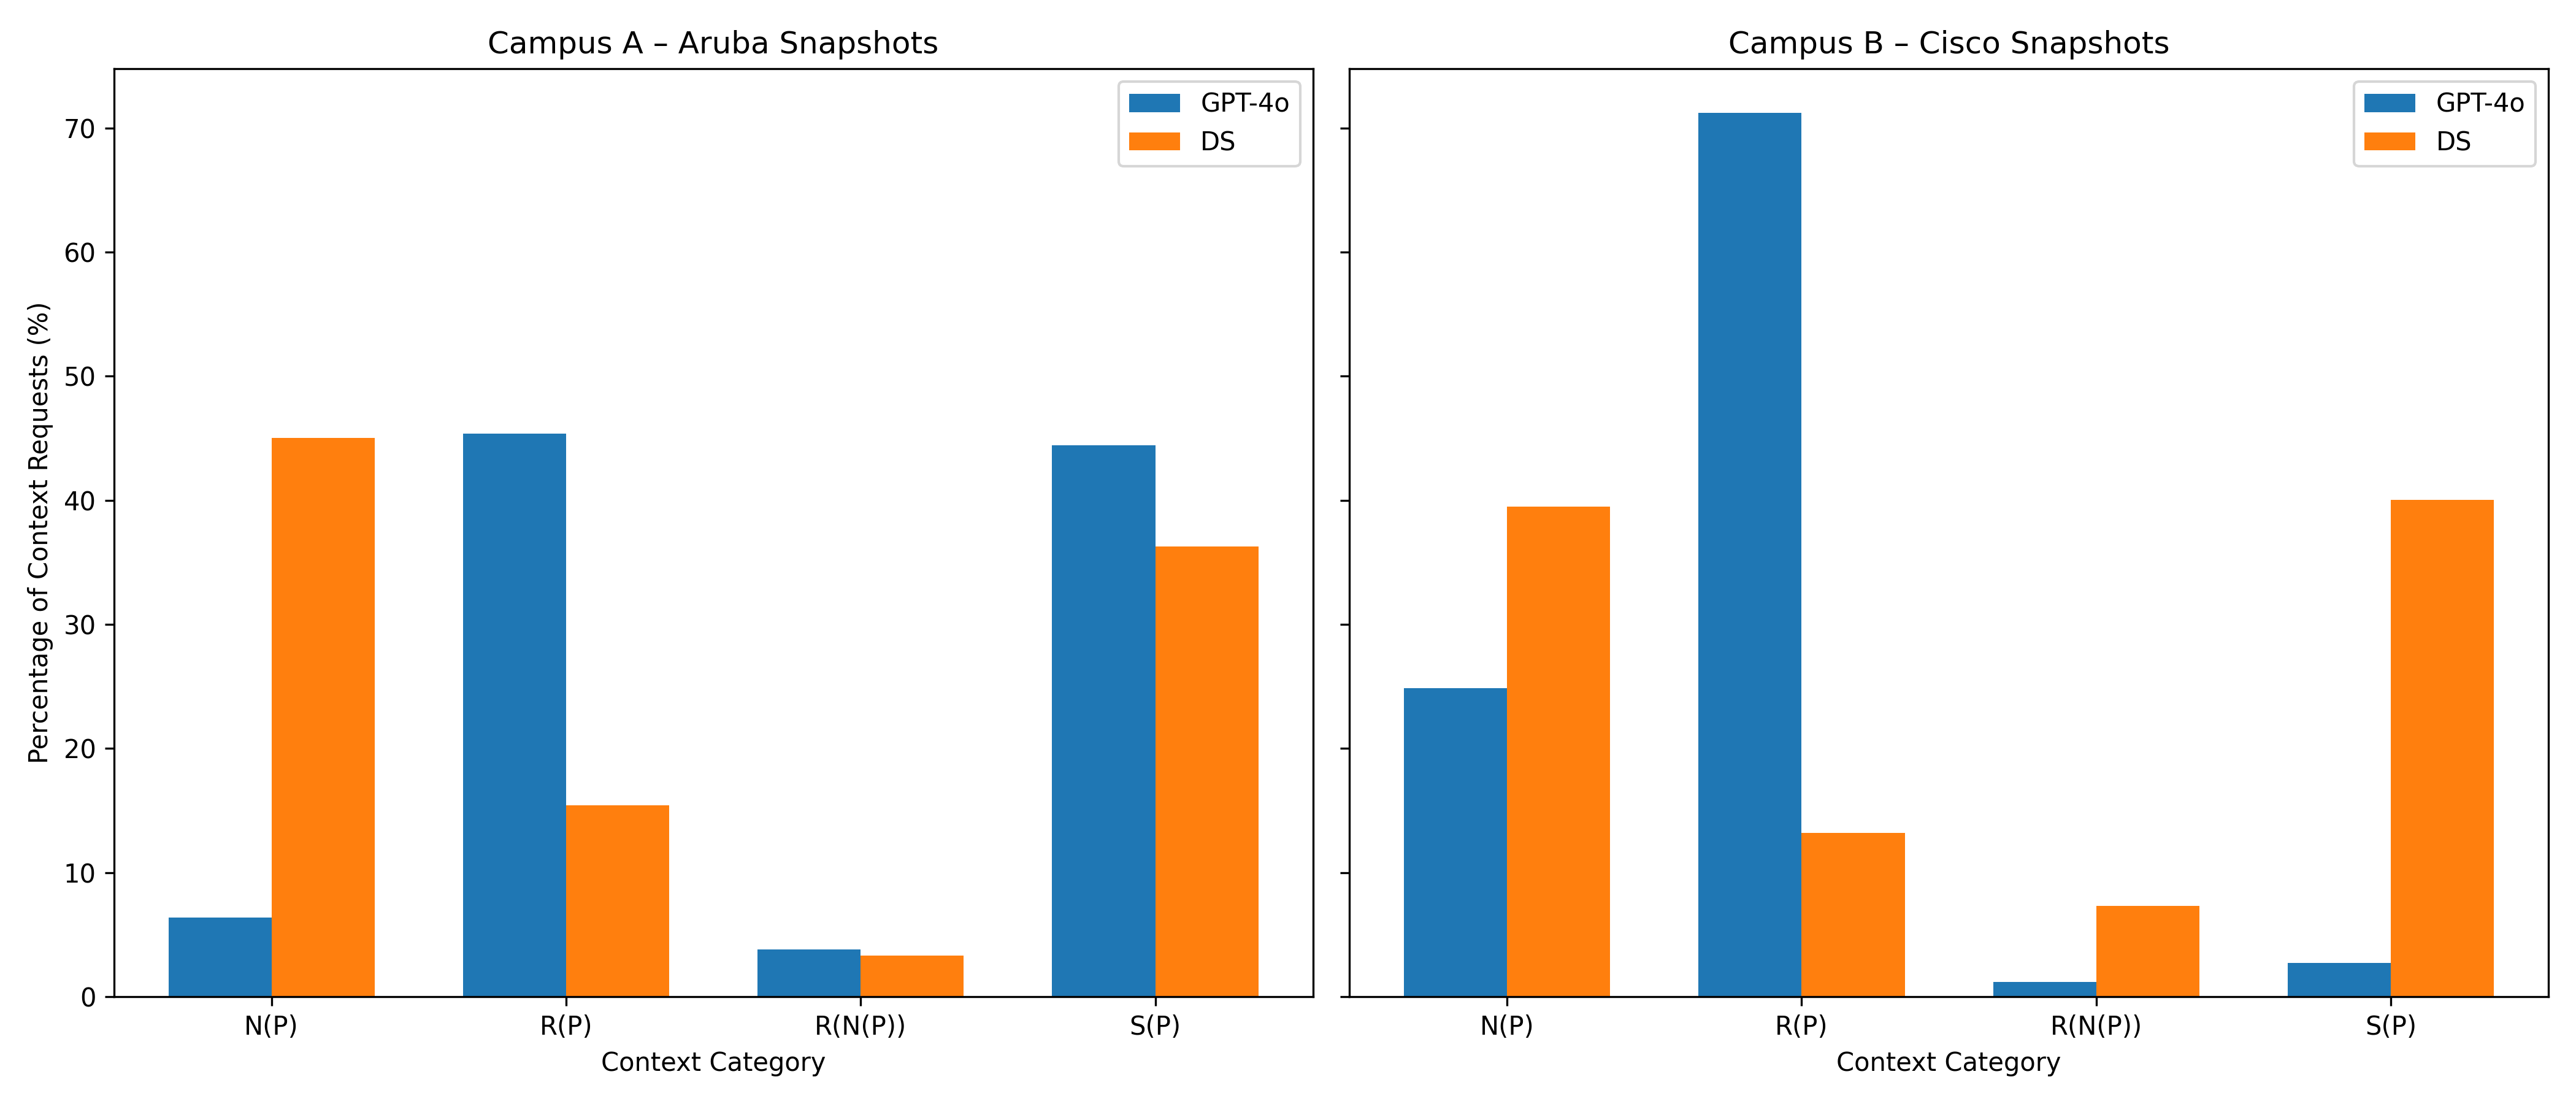
\includegraphics[width=\linewidth]{figs/context_usage_campus_a_b_combined.png}
    \caption{Distribution of context categories requested by GPT-4o and DS, visually highlighting their different analysis strategies.}
    \label{fig:context-usage}
\end{figure*}


\mypara{Implications for Framework Design and Model Choice:}
These observations highlight that the false positives observed in \sysname{} are not artifacts of random noise—they are direct reflections of each model’s interpretive strategy.
This raises an important question about our framework design: in letting the LLM choose its own context to avoid information overload, have we risked the model not requesting \textit{enough} context? To quantify this trade-off, we conducted an ablation study comparing our standard "ask-for-context" approach against a "provide-all-context" method on the challenging Campus B dataset. The results, shown in Table~\ref{tab:ablation_results}, confirm that our design is a justified and effective choice. While providing full context significantly reduced GPT-4o's false positives (from 21 down to 5), it did so at the cost of a threefold increase in prompt size. For DeepSeek, the additional context provided no accuracy benefit, only increasing its computational overhead. This study validates that our iterative approach is a more efficient and effective design.


Ultimately, \sysname{}’s explicit, LLM-driven interface provides a transparent foundation for diagnosing such decisions. For a network operator, the choice of model would depend on their goal: GPT-4o's high-recall approach may be preferable for deep, exploratory audits where finding every potential issue is critical, even at the cost of reviewing false alarms. In contrast, DeepSeek's high-precision approach is better suited for continuous, automated checks where minimizing false positives and operator alerts is the primary concern.

\subsection{How Does \sysname{} Compare to Existing Tools?}

Finally, we compare \sysname{}'s performance against four representative state-of-the-art tools using the synthetic misconfiguration dataset from Internet2. This controlled setting, with its clearly defined ground truth, allows for a direct, feature-by-feature comparison. The tools include:
\begin{itemize}
    \item Two consistency checkers: \textit{Batfish}~\cite{fogel2015general} and \textit{Diffy}~\cite{kakarla2024diffy}.
    \item Two alternative LLM-based approaches: a full-file prompting model (\textit{FFP}) and the partition-based Q\&A model \textit{Ciri}~\cite{lian2023configuration}.
\end{itemize}
For a fair comparison, both FFP and Ciri use the same \textbf{GPT-4o} backend as \sysname{} in this experiment. We do not compare against formal model checkers because no specification of forwarding requirements is available for these networks.

The results in Table~\ref{tab:syn_result} demonstrate that \sysname{} significantly outperforms the other tools in detecting all three types of misconfigurations. It achieves a perfect 16/16 detection rate for erroneous configurations and a 100\% accuracy rate overall. This indicates that \sysname{}'s comprehensive context mining and iterative prompting process effectively identify errors, even in complex D/C cases where other tools struggle.

\begin{table}[t]
\centering
\resizebox{0.8\columnwidth}{!}{
\begin{tabular}{|l|l|c|c|}
\hline
\textbf{Model} & \textbf{Framework Version} & \textbf{False Positives} & \textbf{Avg. Context Tokens} \\
\hline
\multirow{2}{*}{GPT-4o} & \sysname{} (Standard) & 21  & $\sim$ 180 \\
 & \sysname{}-FullContext & 5 & $\sim$ 650 \\
\hline
\multirow{2}{*}{DeepSeek-V3} & \sysname{} (Standard) & 4  & $\sim$ 148 \\
 & \sysname{}-FullContext & 4  & $\sim$ 590 \\
\hline
\end{tabular}
}
\caption{Ablation study results on the Campus B dataset, comparing the standard iterative \sysname{} framework against a version that provides all context by default.}
\label{tab:ablation_results}
\end{table}

\begin{table*}[t]
\centering
\resizebox{\columnwidth}{!}{
\begin{tabular}{|l|l|l|l|l|l|l|}
\hline
\multirow{2}{*}{\textbf{Type}} & \multirow{2}{*}{\textbf{Cases}} & \multicolumn{5}{c|}{\textbf{Number of Detected Misconfigurations}} \\ \cline{3-7} 
&                       & \textbf{\sysname{}} & \textbf{Ciri}& \textbf{FFP} & \textbf{Batfish} & \textbf{Diffy} \\ \hline
Syntax Error & 4 & 4/4 (100\%) & 2/4 (50\%) & 0/4 (0\%) & 3/4 (75\%) & 0/4 (0\%) \\ \hline
Range Error & 4 & 4/4 (100\%) & 2/4 (50\%)& 0/4 (0\%) & 0/4 (0\%) & 0/4 (0\%) \\ \hline
D/C Error& 8 & 8/8 (100\%) & 1/8 (12.5\%) & 0/8 (0\%)& 2/8 (25\%) & 0/8 (0\%) \\ \hline
\multirow{2}{*}{\makecell[{{l}}]{Correct Config\\ Updates}}& \multirow{1}{*}{\makecell[{{l}}]{16}} & \multirow{2}{*}{\makecell[{{l}}]{0/16 (0\%)}} & \multirow{2}{*}{\makecell[{{l}}]{0/16 (0\%)}} & \multirow{2}{*}{\makecell[{{l}}]{13/16 (81.2\%)}}& \multirow{2}{*}{\makecell[{{l}}]{0/16 (0\%)}} & \multirow{2}{*}{\makecell[{{l}}]{0/16 (0\%)}} \\ 
& (False Positives) & & & & & \\ \hline
\textbf{Total Accuracy} & \textbf{32} & \textbf{32/32 (100\%)} & \textbf{21/32 (65.6\%)} & \textbf{19/32 (59.4\%)} & \textbf{21/32 (65.6\%)} & \textbf{16/32 (50\%)} \\ \hline
\end{tabular}}
\caption{Comparison of misconfiguration detection on the synthetic dataset. The "Correct Config Updates" row indicates the number of false positives. Lower is better for that row.}
\label{tab:syn_result}
\end{table*}

\mypara{Comparison Against LLM-based Approaches}
The partition-based GPT model, Ciri, performs reasonably well in detecting syntax and range violations (50\% for both). This success is attributable to the LLM's training on vast amounts of text, including network documentation, which allows it to recognize common, localized structures. However, Ciri lags significantly in detecting D/C issues (12.5\%) because its partitioning approach analyzes configuration sections in isolation, failing to capture the complex interdependencies between distant configuration lines that are crucial for detecting such errors.
Full-File Prompting (FFP) attempts to overcome partitioning by providing the entire configuration in a single query, but it proves even less effective, failing to detect any true misconfigurations. Its primary drawbacks are \textit{token limitations}—where large configurations are truncated—and \textit{context overload}, where excessive information prevents the model from prioritizing relevant details.

By dynamically retrieving only the necessary context based on the LLM's requests (as shown in Table~\ref{tab:syn_configs}), \sysname{} eliminates the fragmentation issues of partition-based methods while avoiding the information saturation problem of FFP. This ensures the model receives a focused yet holistic view of configuration interdependencies, dramatically improving its ability to identify complex misconfigurations.

\mypara{Comparison Against Non-LLM-based Tools}
Batfish performs well on syntax errors (75\% detection rate) but struggles with range violations (0\%) and only partially detects D/C issues (25\%). As a consistency checker, Batfish verifies configurations against a predefined set of best practices and structural rules. This makes it effective at catching explicit errors like missing keywords (which a device CLI might also catch) or references to non-existent groups hard-coded in its rules. However, it is less capable of handling misconfigurations that require deeper contextual reasoning, such as policy conflicts or semantic range violations that are not covered by its rules.

Diffy performs poorly across all misconfiguration types (0\% detection rate). Its data-driven approach focuses on learning common usage patterns and flagging structural anomalies. While our misconfigurations do represent deviations, they are often semantic rather than structural. For instance, an invalid MTU value is numerically incorrect but does not alter the configuration's structure, making it difficult for Diffy’s template-based anomaly detection to capture without a granular understanding of parameter constraints.

Finally, despite varying performance, the majority of the tools—\sysname{}, Batfish, Diffy, and Ciri—successfully marked all 16 correct updates as valid, demonstrating strong capabilities in avoiding false positives. However, FFP failed in this aspect, falsely classifying 13 out of 16 correct updates as misconfigurations. This hallucination likely stems from FFP’s inability to effectively filter relevant information within a large configuration file, leading the model to generate erroneous assessments.

While a direct comparison on the Campus A and B configurations would be valuable, many of the novel issues found by \sysname{} (\eg, ambiguous rate limits, insecure but syntactically valid algorithms) are semantic or policy-related issues that fall outside the designed scope of traditional consistency checkers and pattern-based tools. The synthetic dataset thus provides a fairer and more controlled basis for comparison.
% \section{Discussion and Future Work}
% \label{sec:future}

% \sysname{} has proven effective in improving the detection of routing device misconfigurations, but there are several avenues for further exploration and refinement. One challenge is expanding the framework to better handle large-scale, distributed networks with interdependent routers. These environments often involve complex relationships between devices, and future work could focus on extending \sysname{} to capture and analyze multi-device contexts by default. Incorporating cross-router consistency checks and advanced network-wide policy validation could be valuable enhancements.

% Another area for improvement is reducing false positives while maintaining high detection accuracy. Without a definitive ground truth, distinguishing between true misconfigurations and intentional deviations is inherently challenging. Future work could explore techniques such as refining prompt engineering, incorporating confidence scoring, or leveraging ensemble methods to improve robustness and reduce unnecessary alerts.

% Additionally, enhancing the LLM's ability to process real-time configuration changes is crucial. As networks evolve dynamically, incorporating real-time monitoring data into the context mining process would allow for continuous verification and faster misconfiguration detection. Integrating \sysname{} with network management tools that track operational metrics could provide valuable runtime data, further improving detection accuracy by correlating live data with configuration snapshots.
% Future enhancements can also involve proposing and implementing automated fixes for detected misconfigurations with real-time updates. This would help network operators quickly address issues, streamlining troubleshooting and repairs.


\section{Discussion and Future Work}
\label{sec:future}
A key insight from our work is that the choice of the underlying LLM is not trivial; it reveals a fundamental trade-off between precision and recall. This finding has significant implications for network operators, suggesting that the "best" model may depend on the task—a deep, exploratory audit might favor a high-recall model, while continuous, automated monitoring would benefit from a high-precision one.
A second key insight is that our interactive "ask-for-context" framework is more than a verifier; it is also a diagnostic tool. The context a model requests reveals its underlying reasoning strategy---whether it focuses on local semantics or global patterns. This makes our interactive approach not only more efficient than force-feeding all available context, but also more transparent, providing a crucial window into the model's "thought process" that is essential for building trust in its conclusions.

Building on these insights, future work can proceed in several directions. First, given the precision-recall trade-off, an exciting avenue is to develop an ensemble or meta-LLM framework that could dynamically choose the best model (or combination of models) for a given configuration line or verification task. Second, while our context mining is comprehensive, it could be enriched by incorporating live network state data from sources like BGP routing tables or SNMP, allowing for verification not just of the configuration's snapshots, but also its alignment with the network's real-time operational reality. Finally, the structured output of \sysname{} provides a strong foundation for automated remediation, where the framework could not only detect a misconfiguration but also propose and, with operator approval, apply a validated fix.
\section{Conclusion}
\label{sec:conclusion}


In this paper, we introduced \sysname{}, a framework that enables Large Language Models to analyze network configurations with the nuanced, context-aware reasoning of a human expert. We demonstrated that naive LLM applications fail due to context overload and fragmentation, and we solve this by introducing a two-part mechanism. First, a systematic context mining engine extracts all potentially relevant neighboring, similar, and referenced (both intra--- and cross---device) configurations. Second, an interactive prompting engine engages the LLM in a dialogue, allowing the model to request the specific context it needs for a final, focused analysis. Our evaluation shows that \sysname{} significantly outperforms existing tools, achieves near-perfect accuracy on known errors, and uncovers dozens of previously unknown, real-world misconfigurations. More importantly, our work reveals a critical precision-recall trade-off between different LLM backends, providing a deeper understanding of how these models can be effectively and reliably deployed for network verification.

% In this paper, we introduced \sysname{}, a framework for routing device misconfiguration detection that leverages context-aware iterative prompting to improve LLM accuracy. By systematically extracting relevant context from network configurations
% and following a guided, interactive prompting mechanism, \sysname{} addresses limitations in current model checkers, consistency checkers, and LLM-based models. Through case studies, we demonstrated that \sysname{} outperforms existing methods across different misconfiguration types, ensuring more reliable and scalable network configuration verification.
		\label{endOfBody}
		%-------------------------------------------------------------------------------
		\bibliographystyle{plain}
		\bibliography{citations}
        



\appendix
\section*{Appendix}
\addcontentsline{toc}{section}{Appendix}

\section{Additional Experiment Results}
In this section, we provide additional quantitative and qualitative results to supplement our main findings.

\subsection{Example LLM reasoning for CAIP}\label{subsec:example_llm_reasoning}
\begin{table}[ht]
\centering
\resizebox{\columnwidth}{!}{
\begin{tabular}{|l|l|l|p{8cm}|} % Define a fixed width for the Reason column
\hline
\textbf{Type} & \textbf{Misconfig} & \textbf{errParameter} & \textbf{Reason}\\ \hline

\multirow{3}{*}{\textbf{Syntax}} & \multirow{3}{*}{Missing brace} & \multirow{3}{*}{["<ge-*>"]} & "MTU value for 'family inet' is set to 9174 which is less than the interface MTU value of 9192. The MTU for 'family inet' should not be less than the interface MTU."\\\hline

\multirow{4}{*}{\textbf{Range}} & \multirow{4}{*}{Invalid VLAN ID} & \multirow{3}{*}{["maximum"]} & "The 'maximum' value of 200000 in the configuration line under review significantly exceeds the 'maximum' values of 1000 found in similar configuration lines, indicating a potential range misconfiguration."\\\hline

\multirow{20}{*}{\textbf{D/C}} & \multirow{5}{*}{Policy Conflict} & \multirow{5}{*}{["remove-comms-rt"]} & "There is a conflict in the configuration under term 'remove-comms-rt' where the action 'community add I2CLOUD-EXTENDED-TARGET' is followed by 'community delete I2CLOUD-EXTENDED-TARGET' which are contradictory actions."\\\cline{2-4}

 & \multirow{5}{*}{Disabled Sampling} & \multirow{5}{*}{["inet6"]} & "The family mpls is incorrectly using the IPv6 filter inet6-sample v6filter, which is intended for family inet6 in similar configuration lines. MPLS traffic should have its own specific filter, as the filtering requirements for MPLS are different from those for IPv6."\\\cline{2-4}
 & \multirow{5}{*}{VRF Target Conflict} & \multirow{5}{*}{["target"]} & "The route-distinguisher (RD) in neighoring configurations is set to 11537:381841, while the vrf-target is set to target:11537:313001. These values should typically align, or at least follow certain conventions for mapping VRFs to the correct target instances in MPLS/BGP L2VPN."\\\cline{2-4}
 & \multirow{5}{*}{Incorrect Filter Usage} & \multirow{5}{*}{["input-list"]} & "The family mpls is incorrectly using the IPv6 filter inet6-sample v6filter, which is intended for family inet6 in similar configuration lines. MPLS traffic should have its own specific filter, as the filtering requirements for MPLS are different from those for IPv6."\\\hline
\end{tabular}}
\caption{Example LLM Reasoning for \sysname{}.}
\label{tab:syn_responses}
\end{table}



		\normalfont % Reset to normal font after sloppy
	
	\end{document}
